\documentclass[a4paper,10pt]{article}

\usepackage{float}
\usepackage{graphicx}
\usepackage[english]{babel}
% Package for hyperlinks
%\usepackage[pdftex=true,colorlinks=true,plainpages=false]{hyperref}
\usepackage[pdftex=true,colorlinks=true,linkcolor=blue]{hyperref}

\usepackage{showlabels}

\textwidth 16cm
\oddsidemargin 0cm
\topmargin 0cm
\textheight 22cm

\graphicspath{{./figs/}{../manual/figs/}} % para
%poner las gráficas en un subdirectorio

\usepackage{caption}  % Cambiar Figure: por Figure (sin los dos puntos) en las figure captions
\captionsetup[figure]{labelsep=space}
 \addto\captionsenglish{\renewcommand{\figurename}{Figure }}

\begin{document}
\renewcommand{\showlabelfont}{\small\slshape\color{red}}
\newcommand{\teclapuntos}{
\begin{minipage}[t][1mm][t]{.5cm}{
\vspace*{-10pt}
\includegraphics[width=.5cm]{3dots.png}}
\end{minipage}
}
\newcommand{\openkey}{
\begin{minipage}[t][1mm][t]{1cm}{
\vspace*{-10pt}
\includegraphics[width=1cm]{open.png}}
\end{minipage}
}
\newcommand{\exec}{
\begin{minipage}[t][1mm][t]{.7cm}{
\includegraphics[width=.7cm]{exec.png} }
\end{minipage}
}
\newcommand{\add}{
\begin{minipage}[t][1mm][t]{.5cm}{
\vspace*{-10pt}
\includegraphics[width=.5cm]{add.png} }
\end{minipage}
}
\newcommand{\remove}{
\begin{minipage}[t][1mm][t]{.5cm}{
\vspace*{-10pt}
\includegraphics[width=.5cm]{remove.png} }
\end{minipage}
}
\newcommand{\listados}{
\begin{minipage}[t][1mm][t]{.5cm}{
\vspace*{-10pt}
\includegraphics[width=.5cm]{listados.png} }
\end{minipage}
}
\newcommand{\reset}{
\begin{minipage}[t][1mm][t]{.7cm}{
\includegraphics[width=.7cm]{reset.png} }
\end{minipage}
}
\newcommand{\start}{
\begin{minipage}[t][1mm][t]{.7cm}{
\includegraphics[width=.7cm]{start.png} }
\end{minipage}
}
\newcommand{\stopkeya}{
\begin{minipage}[t][1mm][t]{.7cm}{
\includegraphics[width=.7cm]{stop1.png} }
\end{minipage}
}
\newcommand{\stopkeyb}{
\begin{minipage}[t][1mm][t]{.7cm}{
\includegraphics[width=.7cm]{stop2.png} }
\end{minipage}
}
\newcommand{\minuskey}{
\begin{minipage}[t][1mm][t]{.4cm}{
\vspace*{-10pt}
\includegraphics[width=.4cm]{minuskey.png} }
\end{minipage}
}
\newcommand{\pluskey}{
\begin{minipage}[t][1mm][t]{.35cm}{
\vspace*{-10pt}
\includegraphics[width=.35cm]{pluskey.png} }
\end{minipage}
}
\newcommand{\actualize}{
\begin{minipage}[t][1mm][t]{.7cm}{\includegraphics[width=.7cm]{actualize.png} }
\end{minipage}
}
\newcommand{\toolbN}{
\begin{minipage}[t][1mm][t]{.5cm}{
\vspace*{-10pt}
\includegraphics[width=.5cm]{toolb1.png}}
\end{minipage}
}
\newcommand{\toolbA}{
\begin{minipage}[t][1mm][t]{.5cm}{
\vspace*{-10pt}
\includegraphics[width=.5cm]{toolb2.png}}
\end{minipage}
}
\newcommand{\toolbS}{
\begin{minipage}[t][1mm][t]{.5cm}{
\vspace*{-10pt}
\includegraphics[width=.5cm]{toolb3.png}}
\end{minipage}
}
\newcommand{\toolbP}{
\begin{minipage}[t][1mm][t]{.5cm}{
\vspace*{-10pt}
\includegraphics[width=.5cm]{toolb4.png}}
\end{minipage}
}
\newcommand{\toolbD}{
\begin{minipage}[t][1mm][t]{.5cm}{
\vspace*{-10pt}
\includegraphics[width=.5cm]{toolb5.png}}
\end{minipage}
}
\newcommand{\toolbH}{
\begin{minipage}[t][1mm][t]{.5cm}{
\vspace*{-10pt}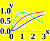
\includegraphics[width=.5cm]{toolb6.png}}
\end{minipage}
}
\newcommand{\toolbB}{
\begin{minipage}[t][1mm][t]{.5cm}{
\vspace*{-10pt}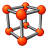
\includegraphics[width=.5cm]{toolb7.png}}
\end{minipage}
}
\newcommand{\toolbQ}{
\begin{minipage}[t][1mm][t]{.5cm}{
\vspace*{-10pt}
\includegraphics[width=.5cm]{toolb8.png}}
\end{minipage}
}
\newcommand{\ggbs}{{\it .ggbs}}
\newcommand{\out}{{\it .out}}
\newcommand{\plt}{{\it .plt}}
\newcommand{\rpd}{{\it .rpd}}


{\large {\bf Quick start-up for DAMQT\_3.2.0} (by R. L\'opez)}

\begin{enumerate}

\item Once the package is installed, run it just writing {\texttt DAMQT320.exe} in any
suitable directory (beware that the executable is accessible by PATH or alike).

\item Choose a language and start DAMQT320 (see fig \ref{fig:1}).

\item When the GUI is open, press the \teclapuntos key placed at
\texttt{Project->Create Project->Import data from} in the left-side menu. Navigate to any
of the samples directories included in the package 
(\texttt{\$DAMQT320)/samples/Molpro/C2H4/}, for
instance; see fig \ref{fig:2}) and double click on file \texttt{C2H4.out}
to launch Molpro's interface to DAMQT320.

\item Press the \exec key. The interface output will appear in the \texttt{Results} pannel 
(see fig \ref{fig:3}).

\item Press on tab \texttt{Atomic densities} on the left side menu and click on
the \exec key. The partition of the density will be carried out and the output
including the multipolar moments of the atomic fragments will be printed in the
viewer (see fig \ref{fig:4}). Now, the {\it .damqt} file containing the fit of the
radial factors of the fragments has been created and all the options will be
accessible. (If your system has not mpi installed, the \texttt{Atomic densities}
menu will look a bit different that in figure; in particular
box labeled \texttt{Parallel computing} will be absent).

\item Press on tab \texttt{Density} on the left side menu, scroll down the menu
with the right vertical rule, and click on
the \exec key to compute the grid for the molecular density. It will take a
few seconds to get the grid computed. Some output will be displayed in the \texttt{Results}
panel (see fig \ref{fig:5}).

\item To compute the molecular density deformations, instead of full density,
check the \texttt{Density deformations} button and press
the \exec key  (see fig \ref{fig:6}).

\item To compute full molecular density in a 2D grid, check radio buttons
\texttt{Full electron density} and \texttt{2D grid},
select the plane \texttt{YZ} which is the molecular plane, and press 
the \exec key  (see fig \ref{fig:7}).
Notice that box following grid type has suitably changed for the 2D grid 
specification.

\item Press on tab \texttt{Electrostatic potential} on the left side menu and
click on the \exec key to compute the grid for the molecular electrostatic
potential (see fig \ref{fig:8}).

\item Check radio button \texttt{2D grid}, select \texttt{YZ} plane, 
and press the \exec key to generate
a 2D grid tabulation (see fig \ref{fig:9}).

\item Press on tab \texttt{Molecular orbitals} on the left side menu. 
In the \texttt{Input data from:}, press the \teclapuntos key to select a file with MO 
an select file \texttt{C2H4.GAorba} (see fig \ref{fig:10})).
Select indices of MO orbitals to be displayed. Indices can be separated by commas.
Ranges of indices separated by hyphens can be also specified (see fig \ref{fig:11}).
Once selected, press the \exec key to generate a grid.

\item Press on tab \texttt{Molecular topography} on the left side menu. Check
the boxes labeled as \texttt{Construct molecular graph} and
\texttt{Construct 3D atomic basin}, and
click on the \exec key to compute the Topography of molecular density (see fig
\ref{fig:12}).

\item Check radio button \texttt{Molecular potential} and press the \exec key 
to compute the Topography of molecular electrostatic potential (see fig \ref{fig:13}).

\item Press on tab \texttt{Mesp sigma hole} on the left side menu.
In the \texttt{Import density from:}, press the \teclapuntos key to select a file with 
a 3D density grid. This grid will be used to generate a density isosurface
with the contour chosen in the box labeled as \texttt{Density value}.
Once selected, press the \exec key to compute the electrostatic potential
on the isosurface (see fig \ref{fig:14}).

\item Press on tab \texttt{Electric field} on the left side menu and
click on the \exec key to compute electric field lines
(see fig \ref{fig:15}).

\item Press on tab \texttt{Density gradient} on the left side menu and
click on the \exec key to compute 3D density gradient lines
(see fig \ref{fig:16}). 

\item Check \texttt{2D grid} button and
in \texttt{2D planes} check \texttt{YZ} plane
to generate density gradient lines on the molecular plane (see fig \ref{fig:17}).

\item Press on tab \texttt{H-F Forces on nuclei} on the left side menu and
click on the \exec key to compute the Hellmann-Feynman forces on nuclei (see fig
\ref{fig:18}).

\item Press on tab \texttt{Radial factors} on the left side menu. Change \texttt{Step}
to 0.02, and choose $l$ and $m$ values.
Select the centers whose radial factors are to be displayed, check
boxes for derivatives and press the \exec key (see fig \ref{fig:19}).

\item Press on tab \texttt{Oriented multipoles} on the left side menu. 
Select the set of oriented multipoles to be computed with the \texttt{lmin} and
\texttt{lmax} spinboxes, the centers defining the plane, and those whose oriented multipoles are to be 
computed. Press the \exec key to compute (see fig \ref{fig:20}).

\item Press on tab \texttt{Zernike-Jacobi density expansion} on the left side menu.
Press the \exec key to compute Canterakis-Zernike expansion of density (see fig \ref{fig:21}).

\item Press on tab \texttt{Zernike-Jacobi density tabulation} on the left side menu.
In the \texttt{Import data from:}, press the \teclapuntos key to select a file with 
a Canterakis Zernike expansion (see fig \ref{fig:22}).
Press the \exec key to compute Canterakis-Zernike expansion of density.

\end{enumerate}

Many of the previous actions, besides the output data printed in the viewer and
stored in \out{ } files, have created files to be visualized with the 2D plotter
or the 3D viewer. For 2D plotting do the following:

\begin{enumerate}
\item Press button \texttt{New 2D Plotter} on the right menu. A window for 2D plotting
will be opened (see fig \ref{fig:23}).

\item To visualize a 2D contour plot, select tab \texttt{Contour plots} and
press the \teclapuntos key to select a file with grid data
(see fig \ref{fig:24}). Open the file and the contour plot will be displayed.
Contour values can be displayed by double clicking on the lines
(see fig \ref{fig:25}).

\item To visualize 2D electric field lines (or density gradient lines), open a new
2D plotter and select tab \texttt{Field lines} and press the \teclapuntos key to select a file 
with grid data (see fig \ref{fig:26}). Open the file and field lines will be displayed.
Check \texttt{Show arrows} box to display arrows on the lines (see fig \ref{fig:27}).
Alternatively, lines can be displayed over the contour plot. To do this, in the plotter
with 2D contour lines, select tab \texttt{Field lines} and proceed as before.
You will be asked to superimpose image (see fig \ref{fig:28}). 
Answering {\it yes} will cause the field lines to be superimposed on the contour 
lines (see fig \ref{fig:29}).

\item To display the MESP sigma hole histogram, open a new 2D plotter
and select the pertaining tab. Import a file with the histogram and carry out 
smoothing if desired (see fig \ref{fig:30}). Several histograms can be 
displayed together. Each curve and its label can be edited by double clicking
on the label (see fig \ref{fig:31}).

\item To display radial factors, open a new 2D plotter and select the 
pertaining tab. Import a file with the radial factors or their derivatives 
(see fig \ref{fig:32}). Several files can be imported in the same plot.
Everytime you import a file, you will be prompted for superimposing
(see fig \ref{fig:33}). Curves and their labels can be edited by 
double clicking on their labels (see fig \ref{fig:34}).

\item Critical points can be superimposed to contour lines and field lines or displayed
alone. Go to the first plotter, which now contains the contour MESP 
and electric field lines and select tab \texttt{Critical points}. Import
the {\it C2H4-cps-v.xyz} file containing MESP critical points.
Increase the balls radii to make the CPs more visible (see fig \ref{fig:35}).

\item Basins frontiers on the plane can be also superimposed in this 2D plot.
To do this, select tab \texttt{Basins} and import {\it C2H4-v.basin2D} file.
Increase pen thickness to make the MESP basins frontiers more visible (see fig \ref{fig:36}).

\item Tab \texttt{Options} contains general options.

\item Tab \texttt{Image capture} allows to save plot to a file. Several formats
are available and resolution can be scaled or user-defined.

\item Tab \texttt{Save/retrieve settings} allows to save current settings to a file
to be retrieved when required.

\end{enumerate}

% Figures 37 to 39 are intendendly skipped (for a possible inclusion of new 2D plot figures)

For 3D visualizations do the following:

\begin{enumerate}

\item  Press button \texttt{New 3D viewer} on the right menu. A window for 3D display
will be opened (see fig \ref{fig:37}). 

\item In the right menu of the window, press button \texttt{Add molecule} and
choose a file with molecular geometry. Choose file {\it C2H4.xyz} in this case 
(see fig \ref{fig:38}) and open it. Use the left mouse button to rotate the
molecule so that the molecular plane coincides with the screen (see fig \ref{fig:39}).

\item Press button \texttt{Geometry measures}, choose \texttt{Distances}
and check \texttt{Show/hide distances in a window} and
{Show/hide distances in the viewer}, Next, while keeping \texttt{shift} key pressed, double click on pairs of atoms
and the distances will be displayed on viewer and in a new window
(see fig \ref{fig:40}). You can repeat the operation selecting \texttt{Angles},
in which case three atoms must be selected, or \texttt{Dihedral angles},
which requires four atoms.

\item Press \texttt{Edit} button to edit molecule. A new window will be opened
with editing options. Press \texttt{3D lines} button and import a file
with lines. Choose file {\it C2H4.cam} (see fig \ref{fig:41}).
Increase arrows length and width to make them visible (see fig \ref{fig:42}).
Whenever the molecule editor is hidden by the viewer, it can be 
brought to forefront by pressing the \texttt{Edit} button.

\item Press \texttt{Critical points} button and inmport a file with
MESP CPs, choose file {\it C2H4-cps-v.xyz}. Increase balls radii 
and slightly rotate the molecule to better visualize the CPs
(see fig \ref{fig:43}).

\item Uncheck \texttt{Show lines} box and press \texttt{Hide 3D lines manager},
and uncheck (?,?) CP boxes and press \texttt{Hide critical points manager}
to hide lines and CPs.

\item Press \texttt{Add surface} button and import a file with a surface.
Choose file {\it C2H4-d\_0.10E-02.sgh} which contains the MESP
values on the density isosurface of contour 0.001. A spectrogram of MESP 
will be displayed on the isosurface (see fig \ref{fig:44}).

\item In \texttt{Loaded surfaces} press the \texttt{Edit} button placed
on the right of the surface file name. A menu for editing the 
surface will be displayed. In the menu, check the \texttt{Local maxima} and
\texttt{Local minima} boxes. New options will appear in the men. Check
\texttt{Show MESP values} box. Local extrema will be displayed with
their MESP values (see fig \ref{fig:45}). 

\item In the surface editor, change the \texttt{Surface type}
to \texttt{Wire frame}, check the box \texttt{Translucence correction}
and move the slider \texttt{Opacity} to a value slightly lower than 100
to change surface look (see fig \ref{fig:46}). 

\item Check box \texttt{Only selected extrema}. CPs indices, symbols and 
MESP values will disappear. To make them visible in a given CP, double click 
on it (see fig \ref{fig:47}).

\item Press button \texttt{Close} to close the surface editor and \texttt{Hide}
button to hide surface. Then, press button \texttt{Add grid for isosurfaces}
and choose a file with a 3D grid tabulation. Choose file {\it C2H4-v.plt}
which contains a tabulation of MESP on a 3D grid. A menu for adding isosurfaces
will be displayed. Press button \texttt{Add surface} and next \texttt{Edit}.
An editor will be displayed for the isosurface. Choose a value in the box and
press {\it Enter} key or, alternatively, move the slider. The isosurface will
be displayed. Check {\it wire frame} option if desired (see fig \ref{fig:48}).

\end{enumerate}

\newpage

For cluster optimization

\begin{enumerate}

\item Remove or hide displayed surfaces. 

\item Add one more C$_2$H$_4$ molecule in the canvas (see fig \ref{fig:49}).

\item Deactivate the first C$_2$H$_4$ molecule (host) and move the second one (guest) to a 
suitable position. Display some distances to check the relative positions of molecules
and press the \texttt{Optimize cluster} button
(see fig \ref{fig:50}).

\item In the new menu, choose a name for the cluster files and, selecting the option
\texttt{Choose guests from canvas} (see fig \ref{fig:51}).

\item Select the charge model for the atoms in guests. If Open Babel is 
installed and working, charges can be obtained with any of the models 
built in that Open Babel. The available models depend on the Open Babel
version, and are displayed in a ComboBox that is displayed when the button 
\texttt{Open  Babel} is checked. Alternatively, charges can be
supplied by the user checking the \texttt{User supplied} button 
and pressing the \texttt{Import} button. A navigation window is opened for 
loading a suitable file with charges (see fig \ref{fig:52}). By default, a 
files with extension {\it mltmod} will appear in the window. 
Charges generated by DAMQT can be imported from these files. 
Alternatively, charges can be loaded from any suitable file
containing {\it atom symbols} and 
{\it charges} (one pair per line).

\item Press the \texttt{Edit} button to check that the charges have been
correctly loaded. A window will appear with the charges currently chosen
(see fig \ref{fig:52}). Charge values can be edited in the boxes if 
desired.


\item In the new menu, choose a name for the cluster files and, selecting the option
\texttt{Choose guests from canvas}, press the \texttt{Exec} button (see fig \ref{fig:53}).

\item Wait until the message of cluster optimization finished appears (see fig \ref{fig:54}).

\item Display some distances to check the relative positions of molecules, select the file with
the cluster optimization frames, move the system to change the point of view if desired,
and press the \texttt{Replay} button to animate the optimization process (see fig \ref{fig:55}). 
During animation, the point of view can be changed by interactively rotating or translating the cluster.

\item Remove the cluster from the viewer (see fig \ref{fig:56}) 
and restore the guest molecule to its initial position (see fig \ref{fig:57}).

\item Edit the host molecule and load its MESP critical points (CP), 
keep only $(3,+3)$ CP selected and display CP symbols
(see fig \ref{fig:58}).

\item Check the option \texttt{Only selected CPs}, deactivate the 
guest molecule and activate the host. Rotate the host to see 
the CP and double click on one of them to select (see fig \ref{fig:59}).

\item In the cluster optimization menu, change the name of the cluster files, 
check the options \texttt{Use template for guests}
and \texttt{Only selected CPs}, and press the \texttt{Exec} button to carry out optimization using
CP for starting guest positions (see fig \ref{fig:60}).

\item Wait until optimization finishes. Load the file with frames, 
change the point of view if desired, display some distances and press
\texttt{Replay button} to animate the optimization process (see fig \ref{fig:61}).

\item Check the \texttt{Record optimization} option. Verify that the command for creating 
movie is correct (\texttt{fframe} must be installed and accessible in your system
if this is the program chosen for this purpose). Select a name for the movie file and
the option \texttt{Remove frame files at end} unless you want to keep the PNG
files corresponding to the single frames (see fig \ref{fig:62}). 
Repeat animation by pressing \texttt{Replay} and wait until recording ends. 
An {\it *.mp4} file will be generated that can be reproduced
with VLC, for instance. (Some multimedia programs, such as MSWindows multimedia,
are unable to reproduce this file issuing format incompatibility).




\end{enumerate}

You can test the different options at your will using this sample deck or any
other included in the package.

\newpage

\begin{minipage}{.5\linewidth}
\begin{figure}[H]
\caption{\label{fig:1}}
\begin{center}
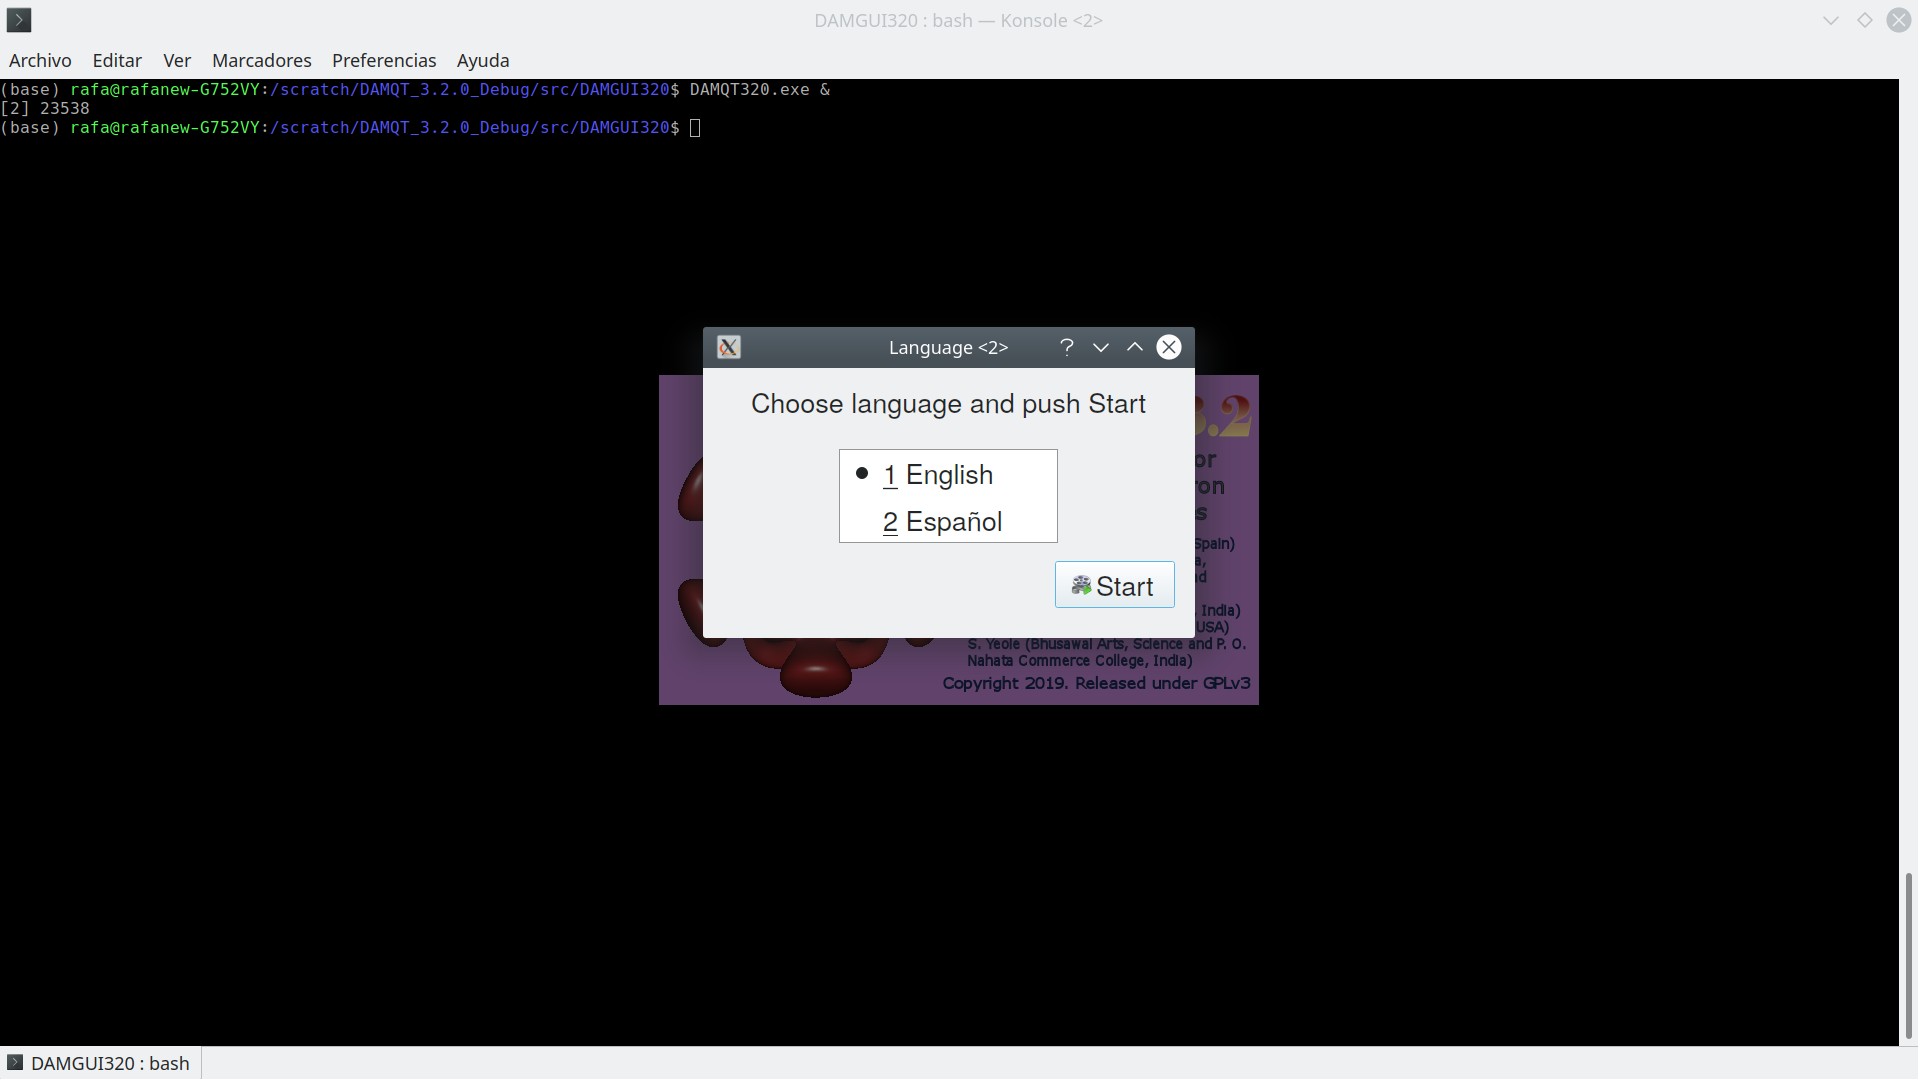
\includegraphics[width=0.95\linewidth]{damqt_QS_fig1.png}
\end{center}
\end{figure} 
\end{minipage}
\begin{minipage}{.5\linewidth}
\begin{figure}[H]
\caption{\label{fig:2}}
\begin{center}
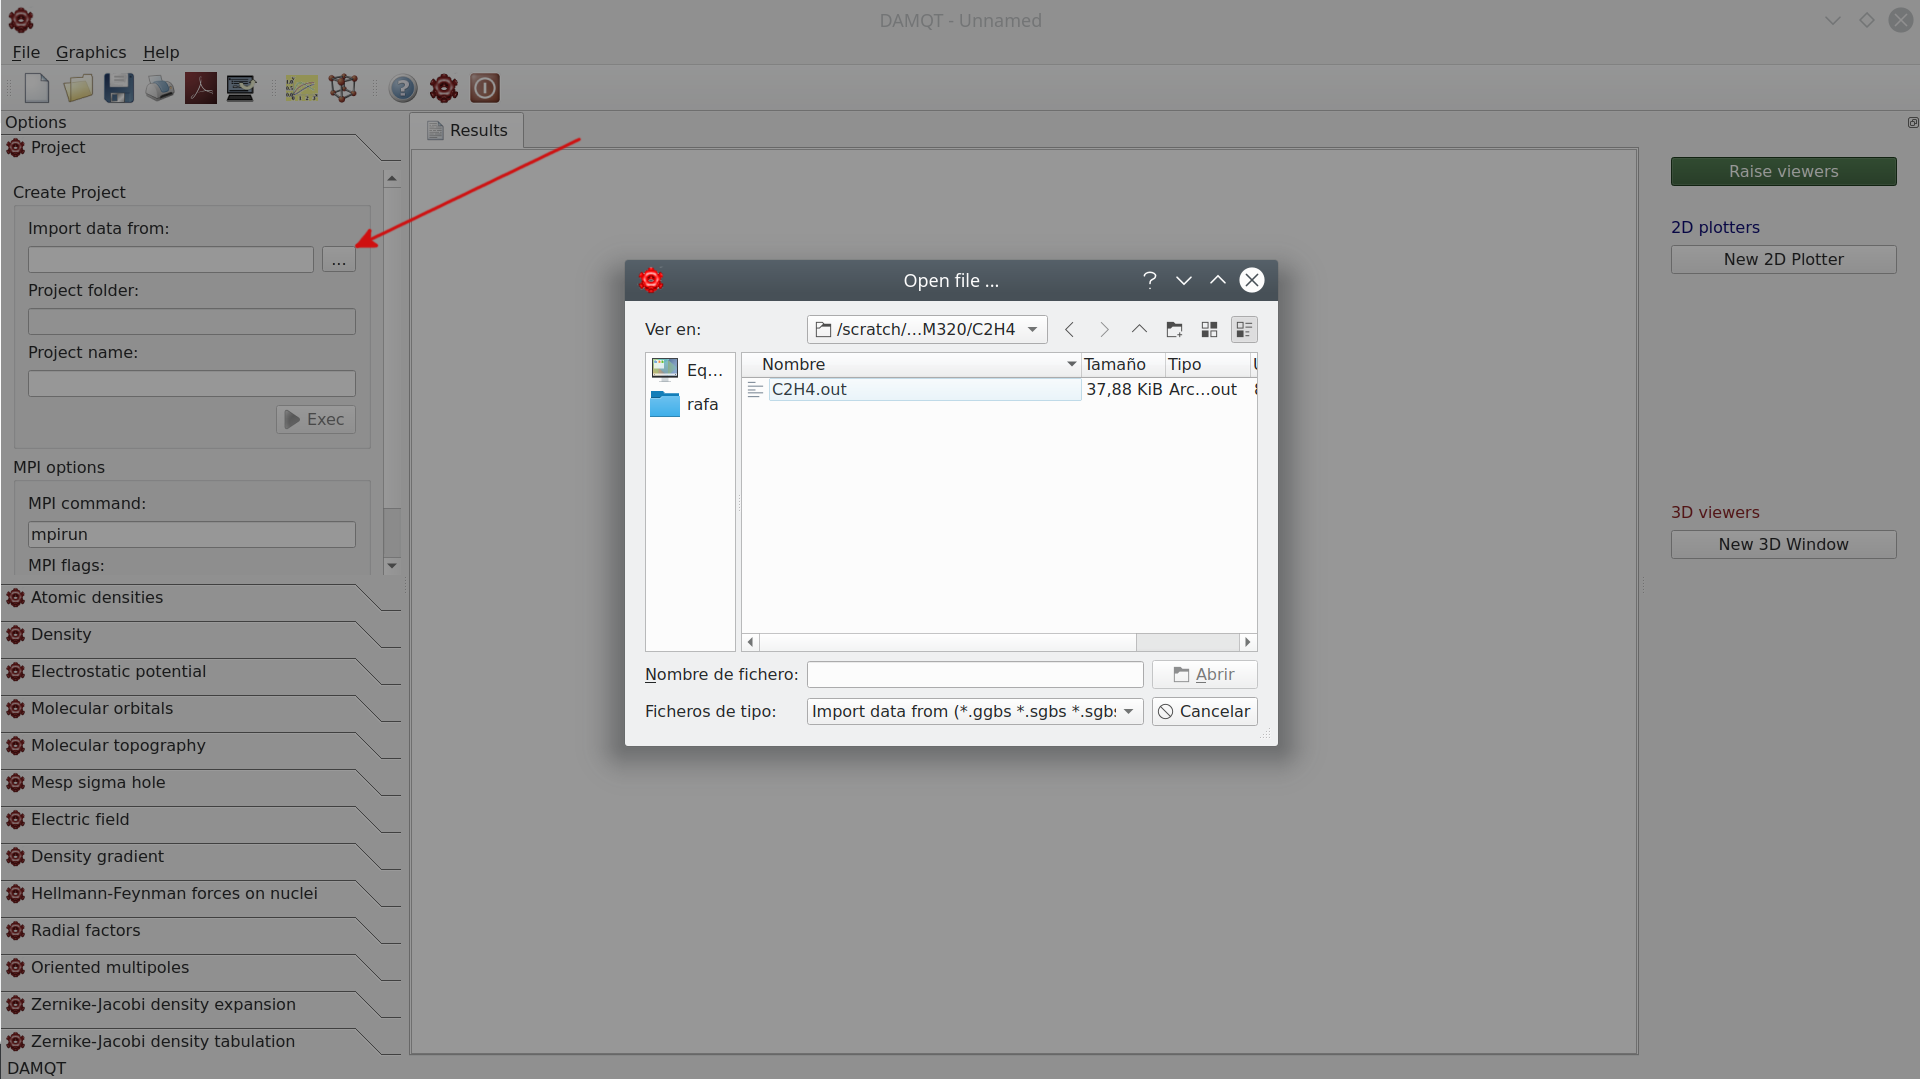
\includegraphics[width=0.95\linewidth]{damqt_QS_fig2.png}
\end{center}
\end{figure} 
\end{minipage}

\begin{minipage}{.5\linewidth}
\begin{figure}[H]
\caption{\label{fig:3}}
\begin{center}
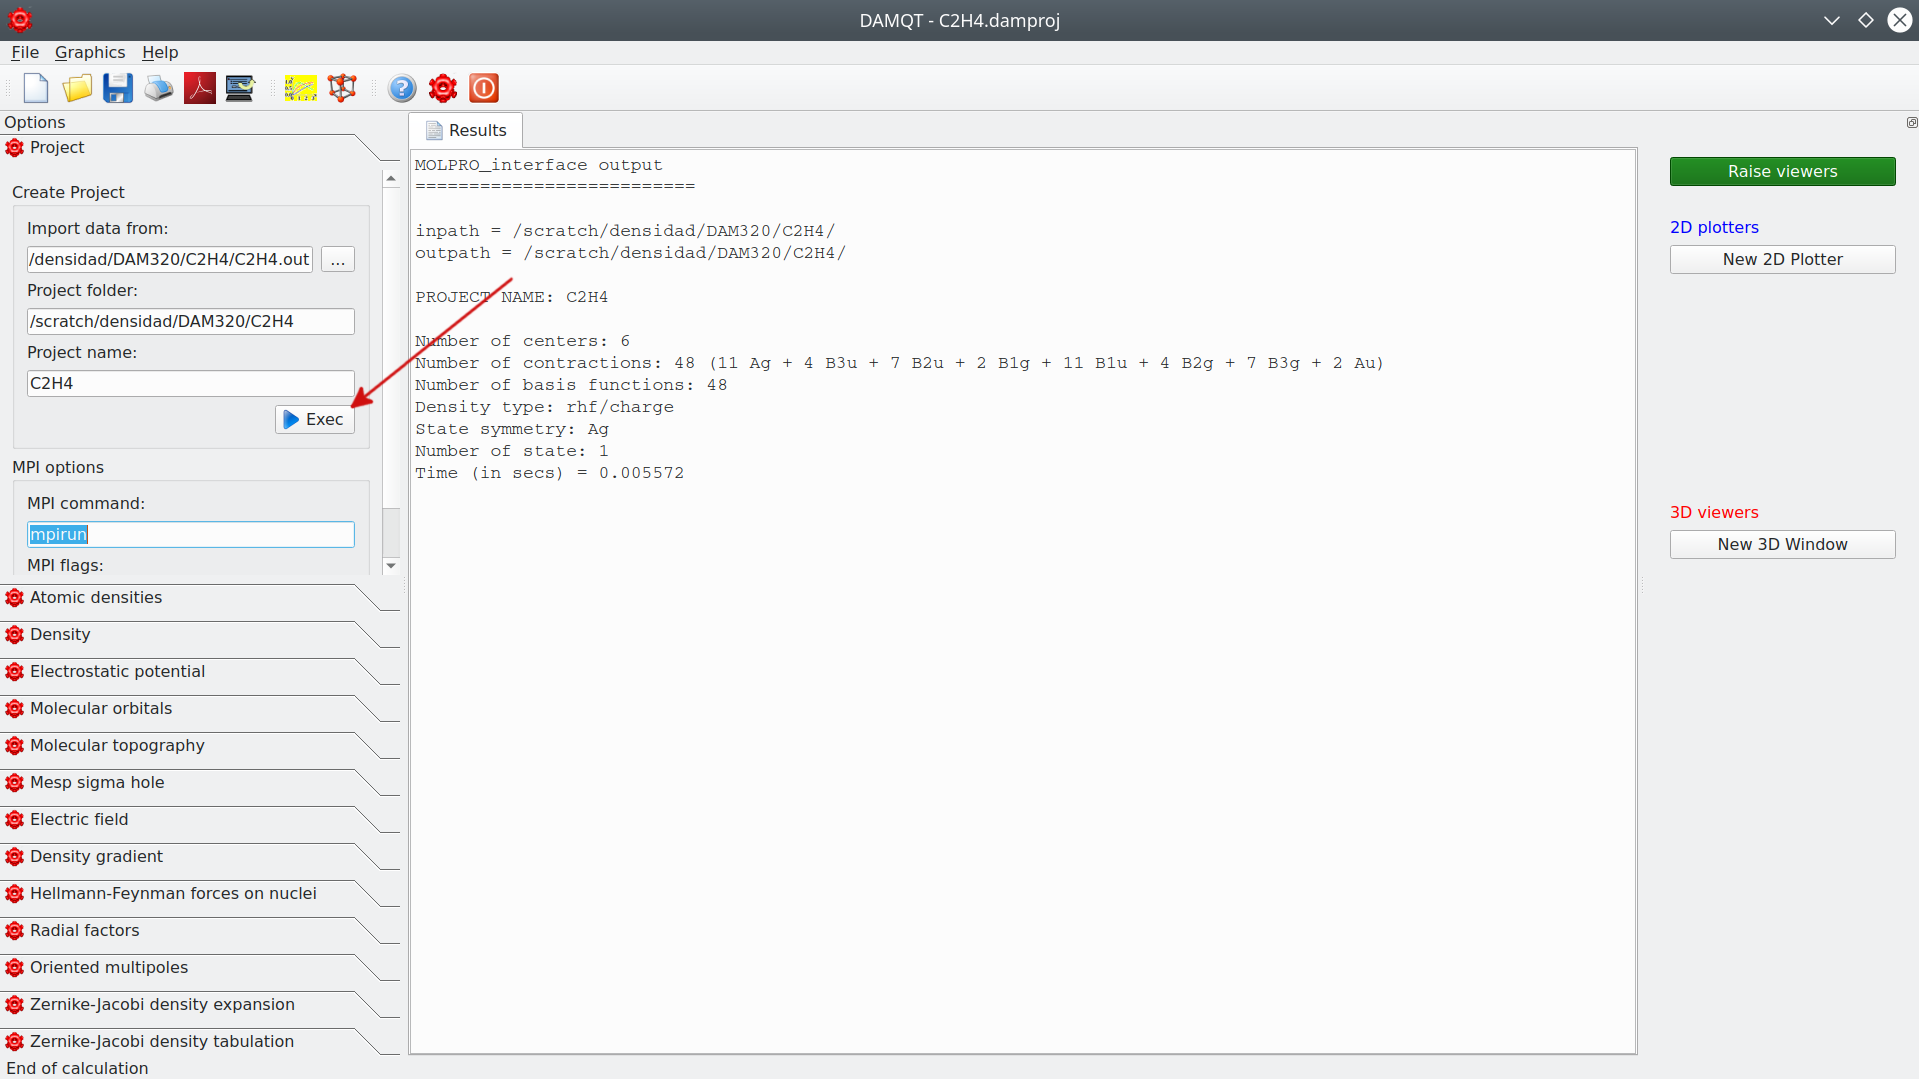
\includegraphics[width=0.95\linewidth]{damqt_QS_fig3.png}
\end{center}
\end{figure} 
\end{minipage}
\begin{minipage}{.5\linewidth}
\begin{figure}[H]
\caption{\label{fig:4}}
\begin{center}
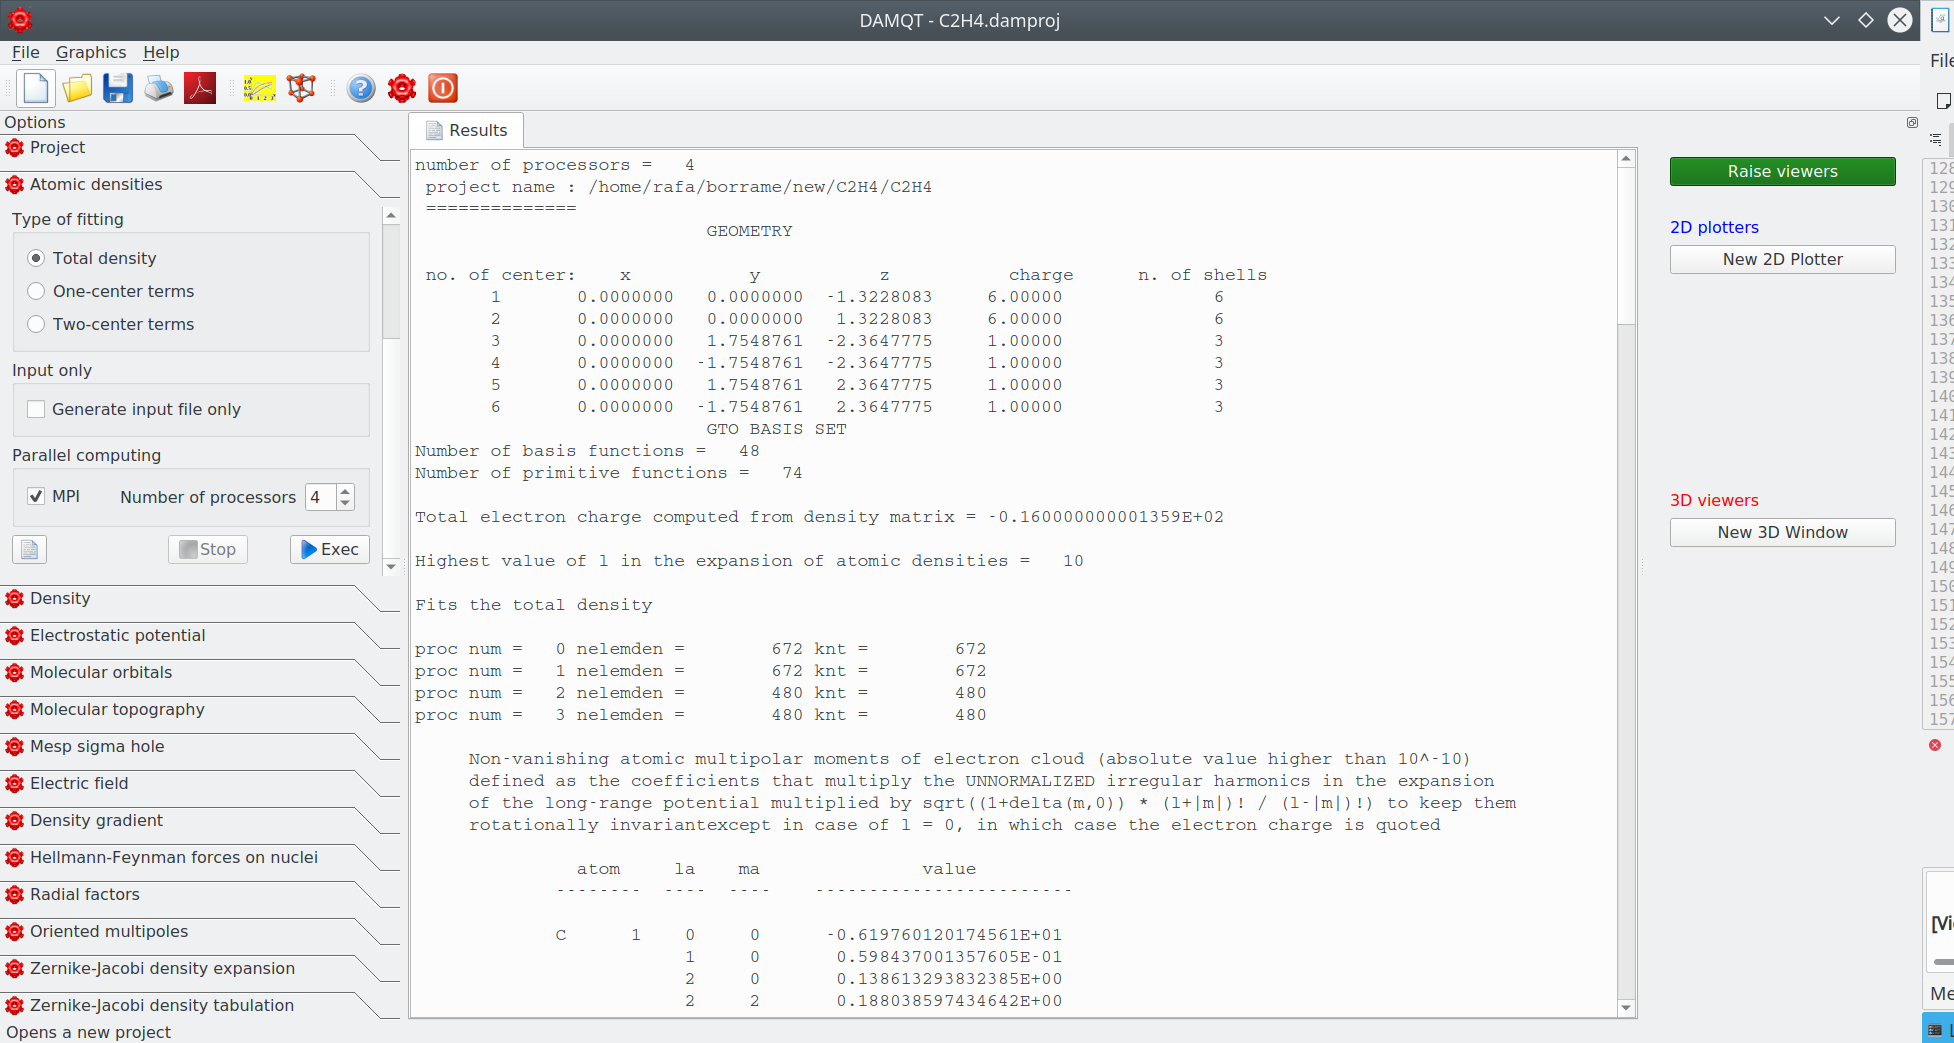
\includegraphics[width=0.95\linewidth]{damqt_QS_fig4.png}
\end{center}
\end{figure} 
\end{minipage}

\begin{minipage}{.5\linewidth}
\begin{figure}[H]
\caption{\label{fig:5}}
\begin{center}
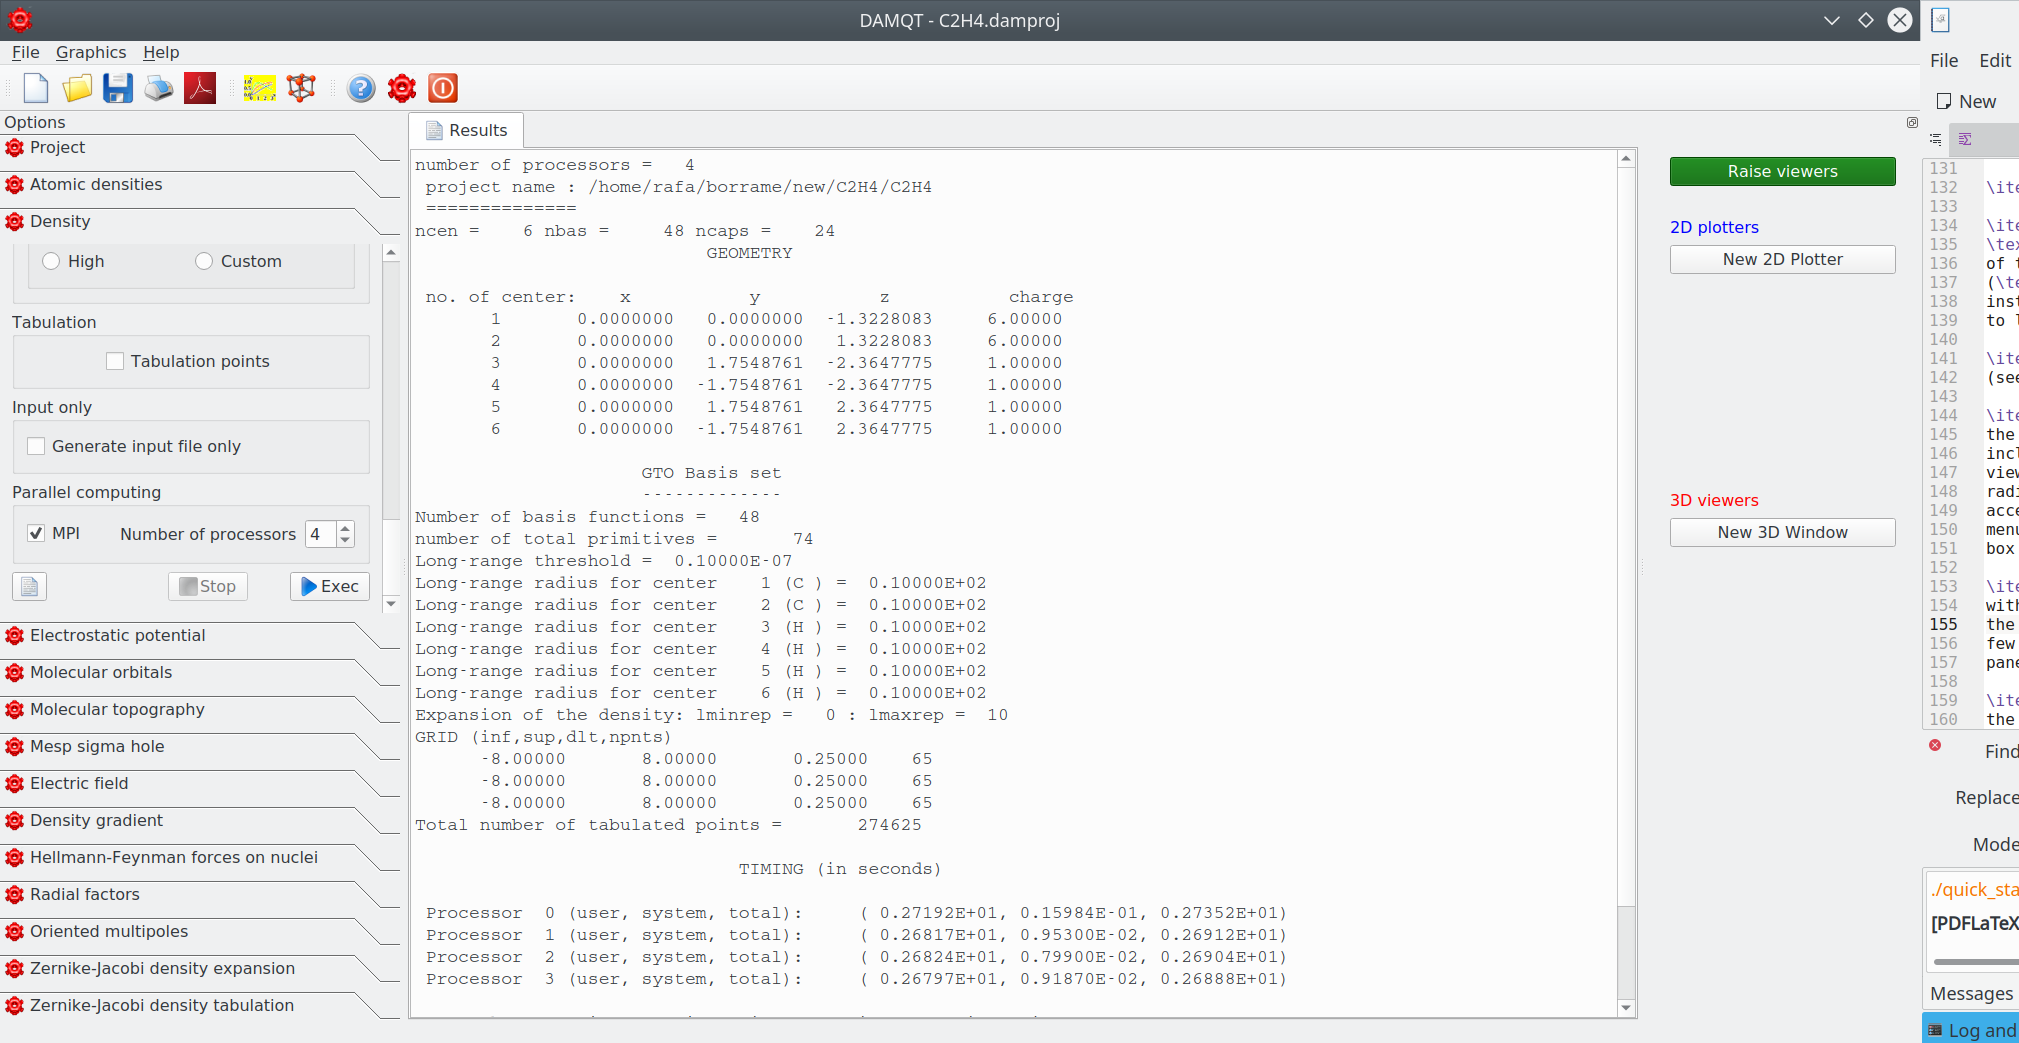
\includegraphics[width=0.95\linewidth]{damqt_QS_fig5.png}
\end{center}
\end{figure} 
\end{minipage}
\begin{minipage}{.5\linewidth}
\begin{figure}[H]
\caption{\label{fig:6}}
\begin{center}
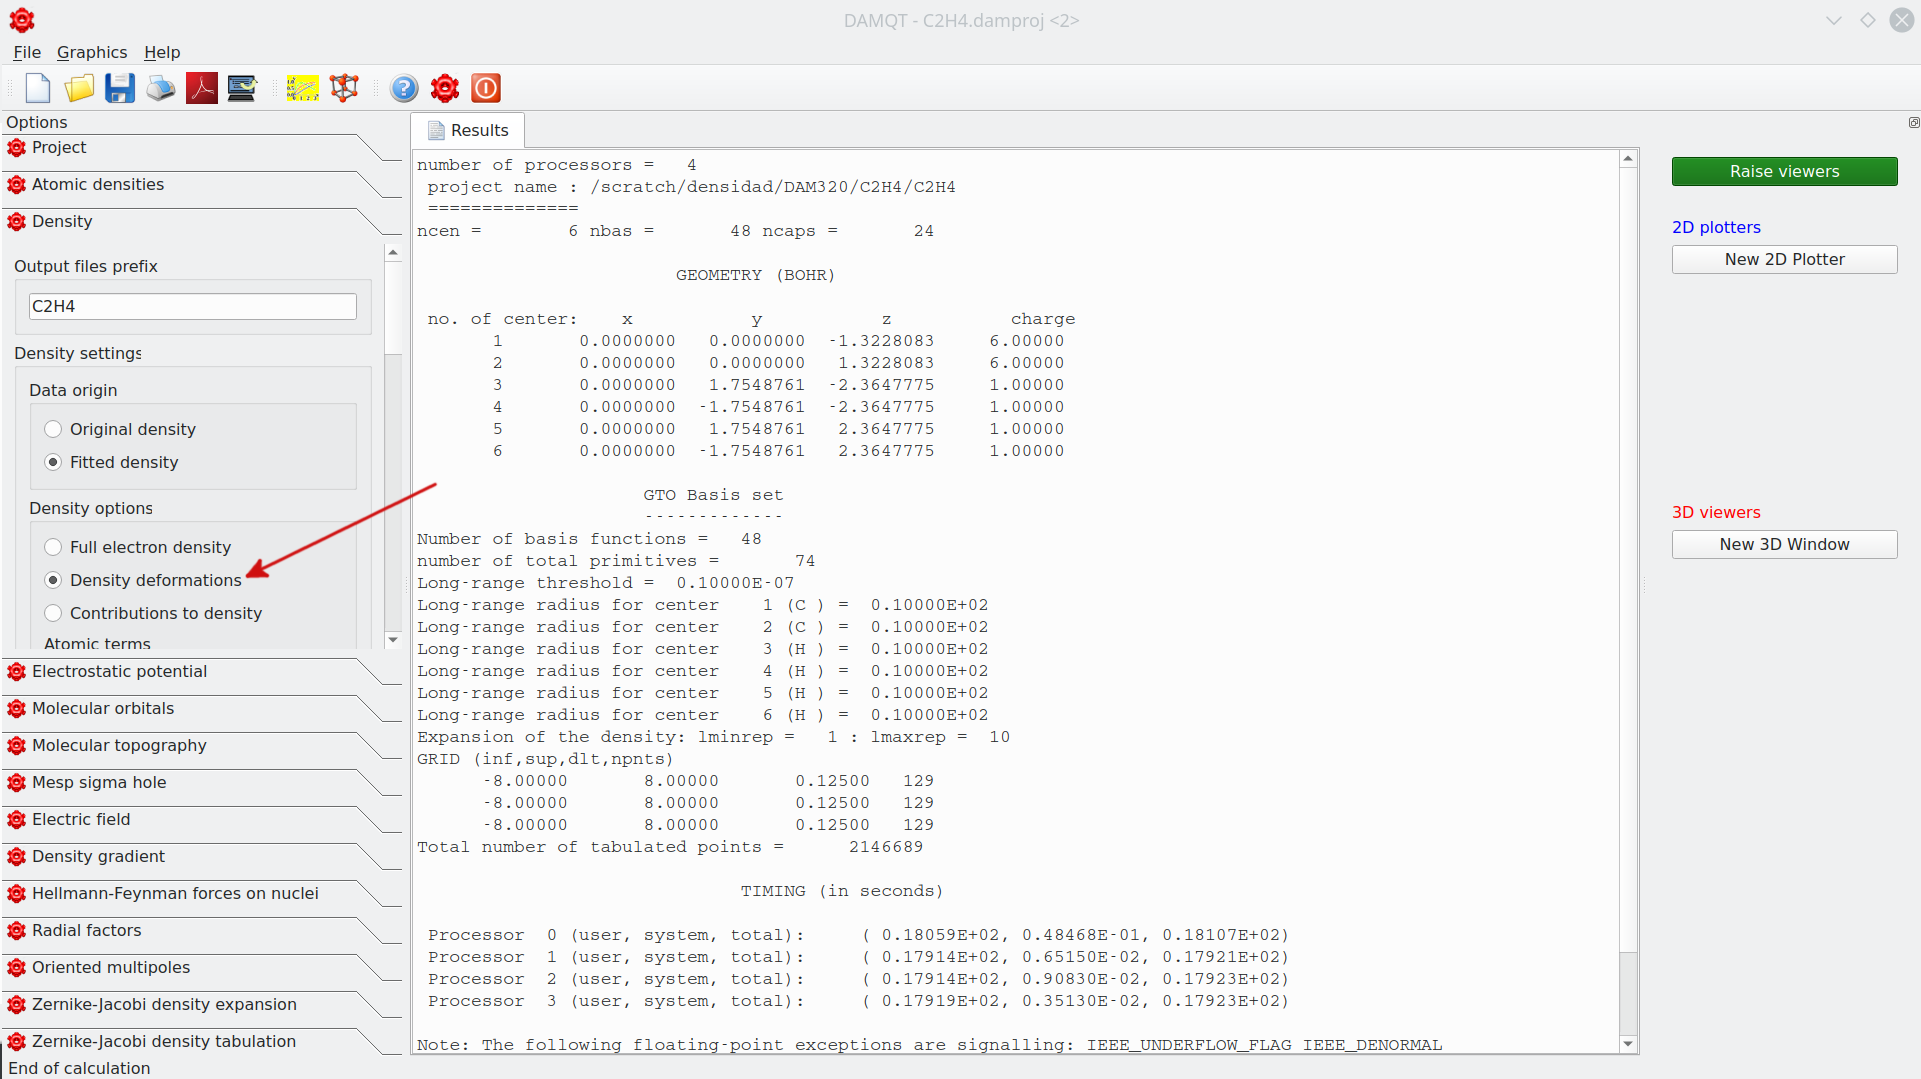
\includegraphics[width=0.95\linewidth]{damqt_QS_fig6.png}
\end{center}
\end{figure} 
\end{minipage}

\begin{minipage}{.5\linewidth}
\begin{figure}[H]
\caption{\label{fig:7}}
\begin{center}
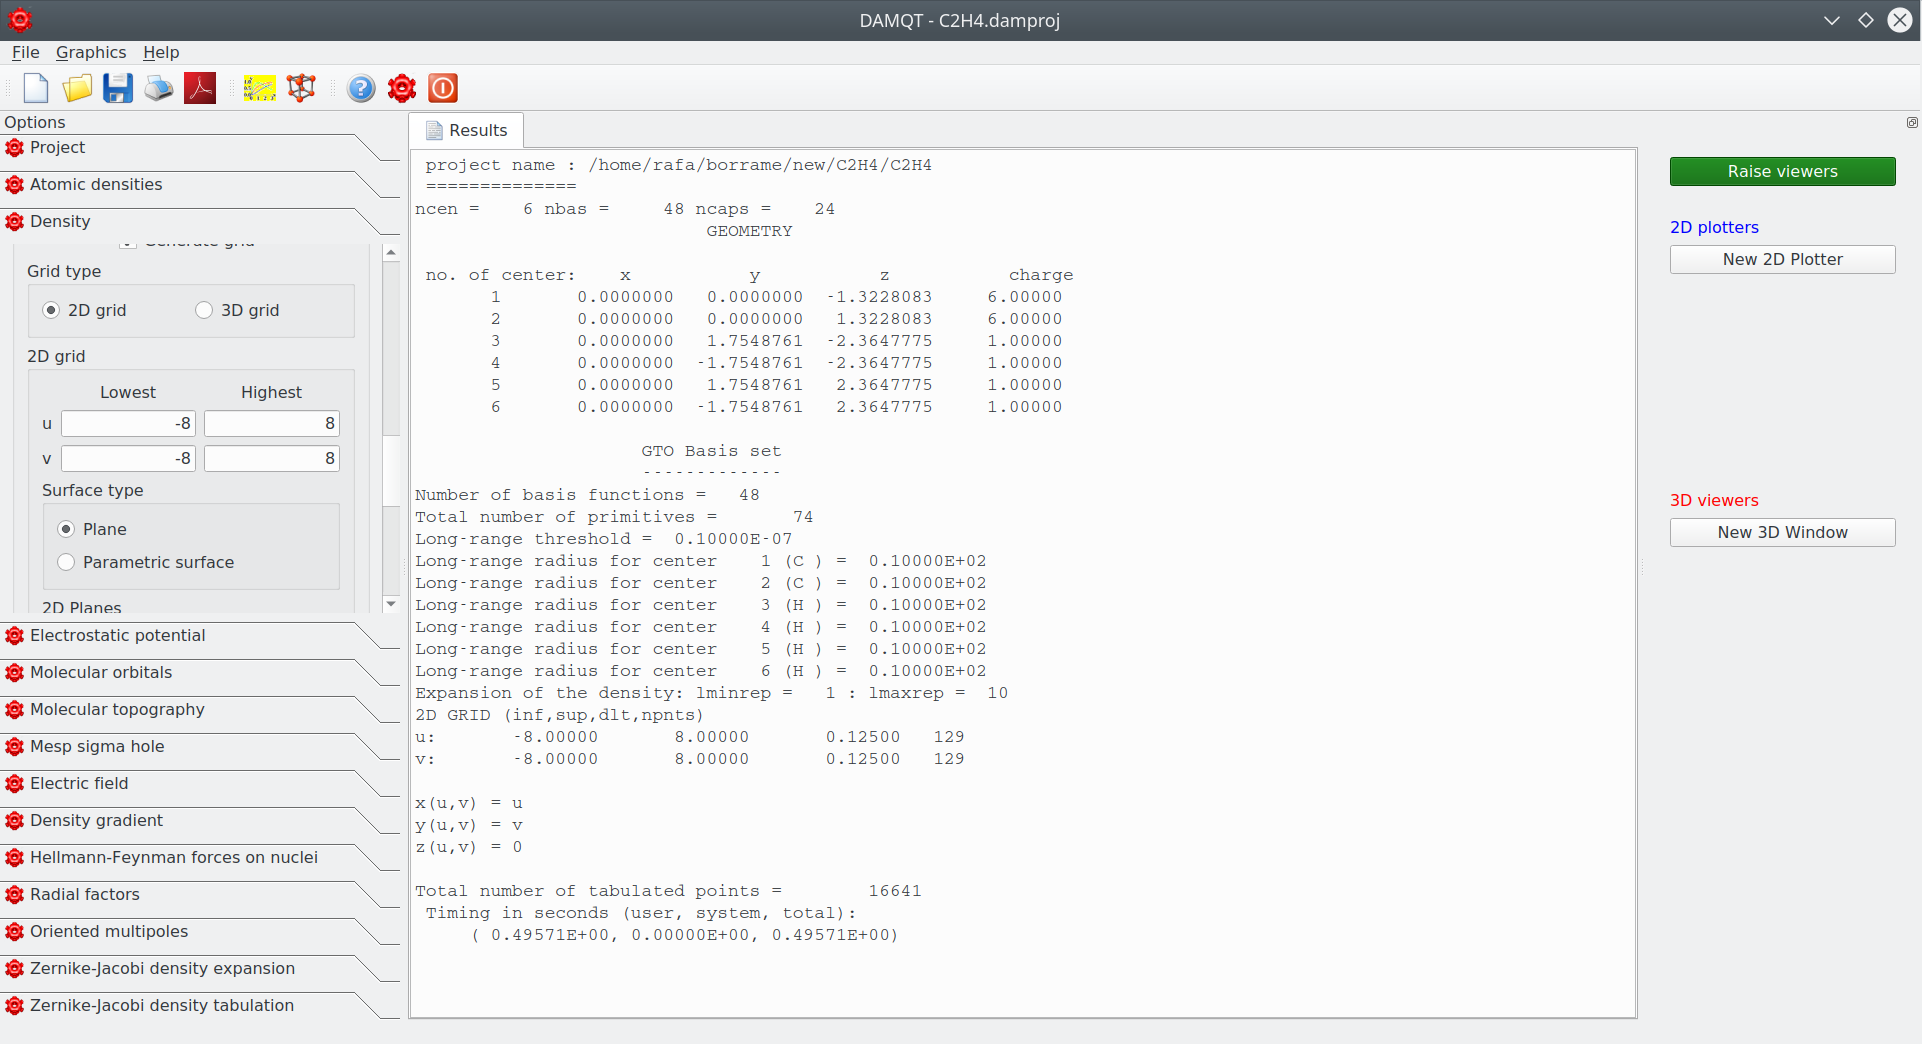
\includegraphics[width=0.95\linewidth]{damqt_QS_fig7.png}
\end{center}
\end{figure} 
\end{minipage}
\begin{minipage}{.5\linewidth}
\begin{figure}[H]
\caption{\label{fig:8}}
\begin{center}
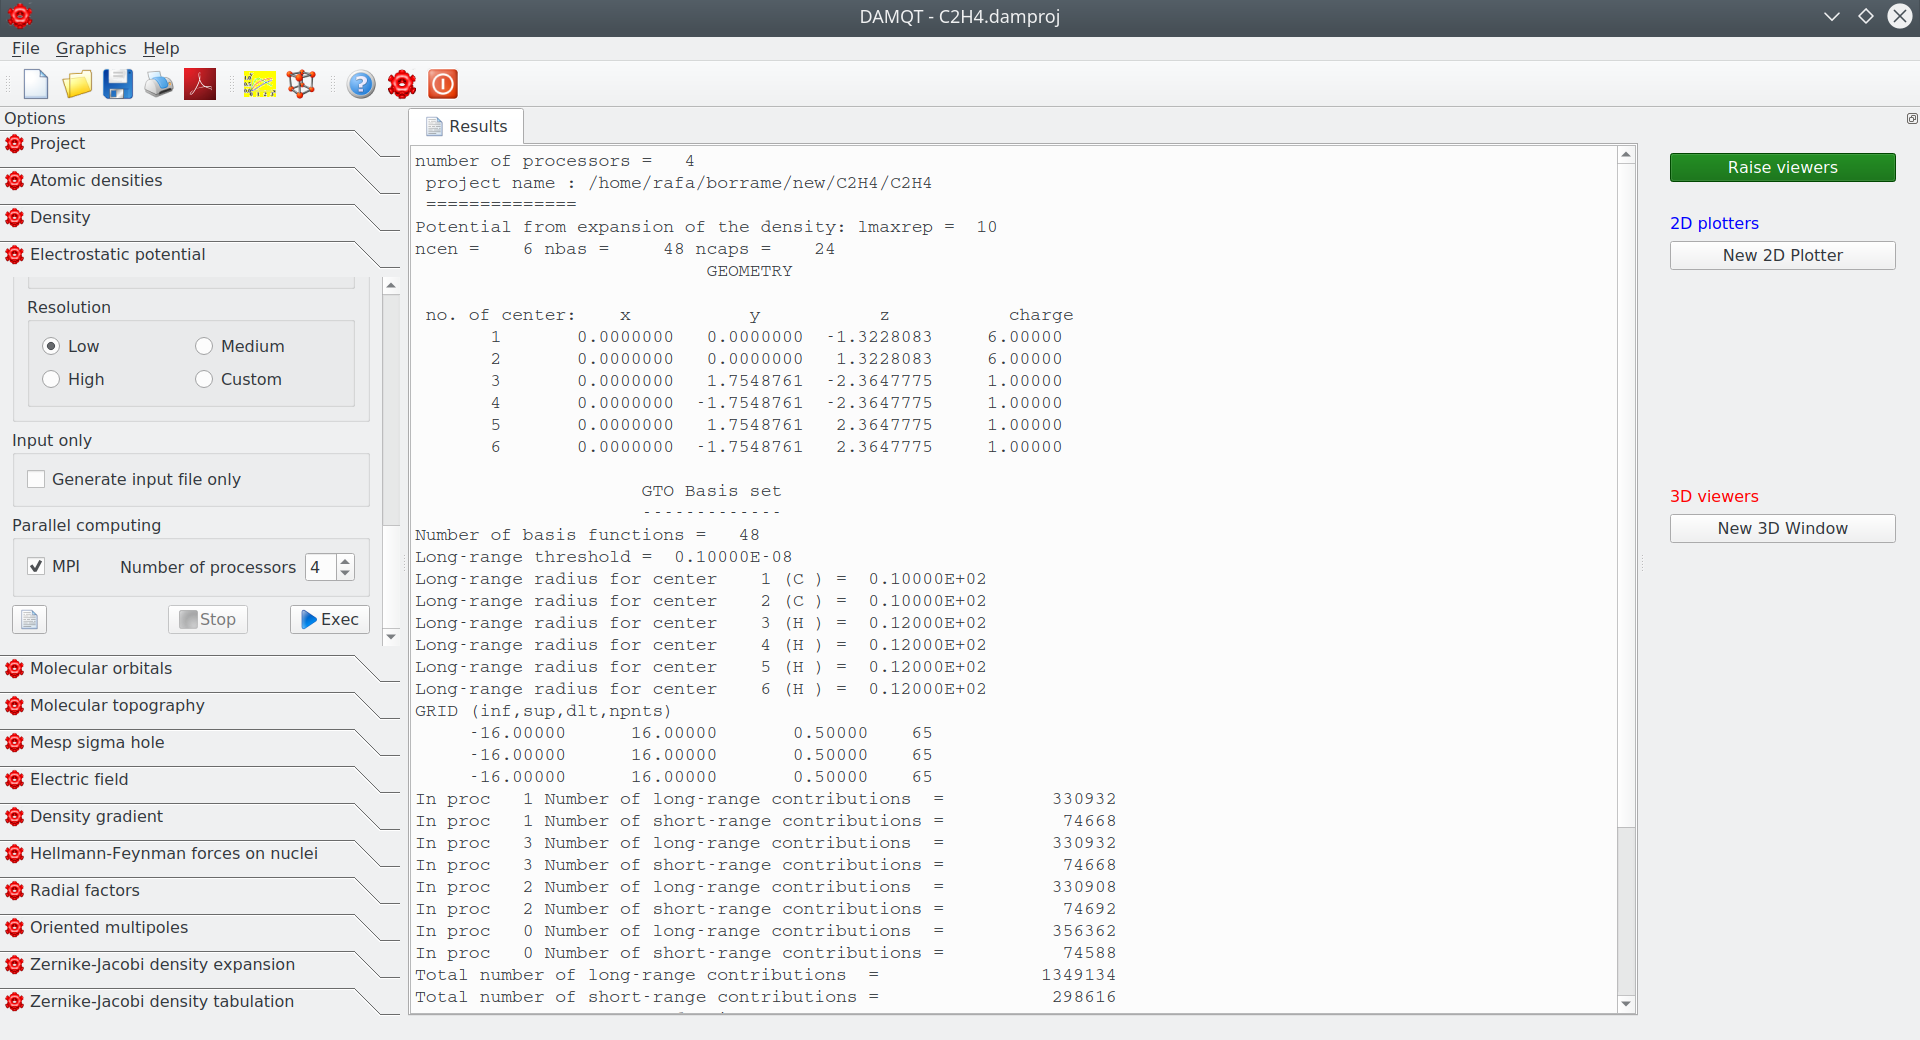
\includegraphics[width=0.95\linewidth]{damqt_QS_fig8.png}
\end{center}
\end{figure} 
\end{minipage}

\begin{minipage}{.5\linewidth}
\begin{figure}[H]
\caption{\label{fig:9}}
\begin{center}
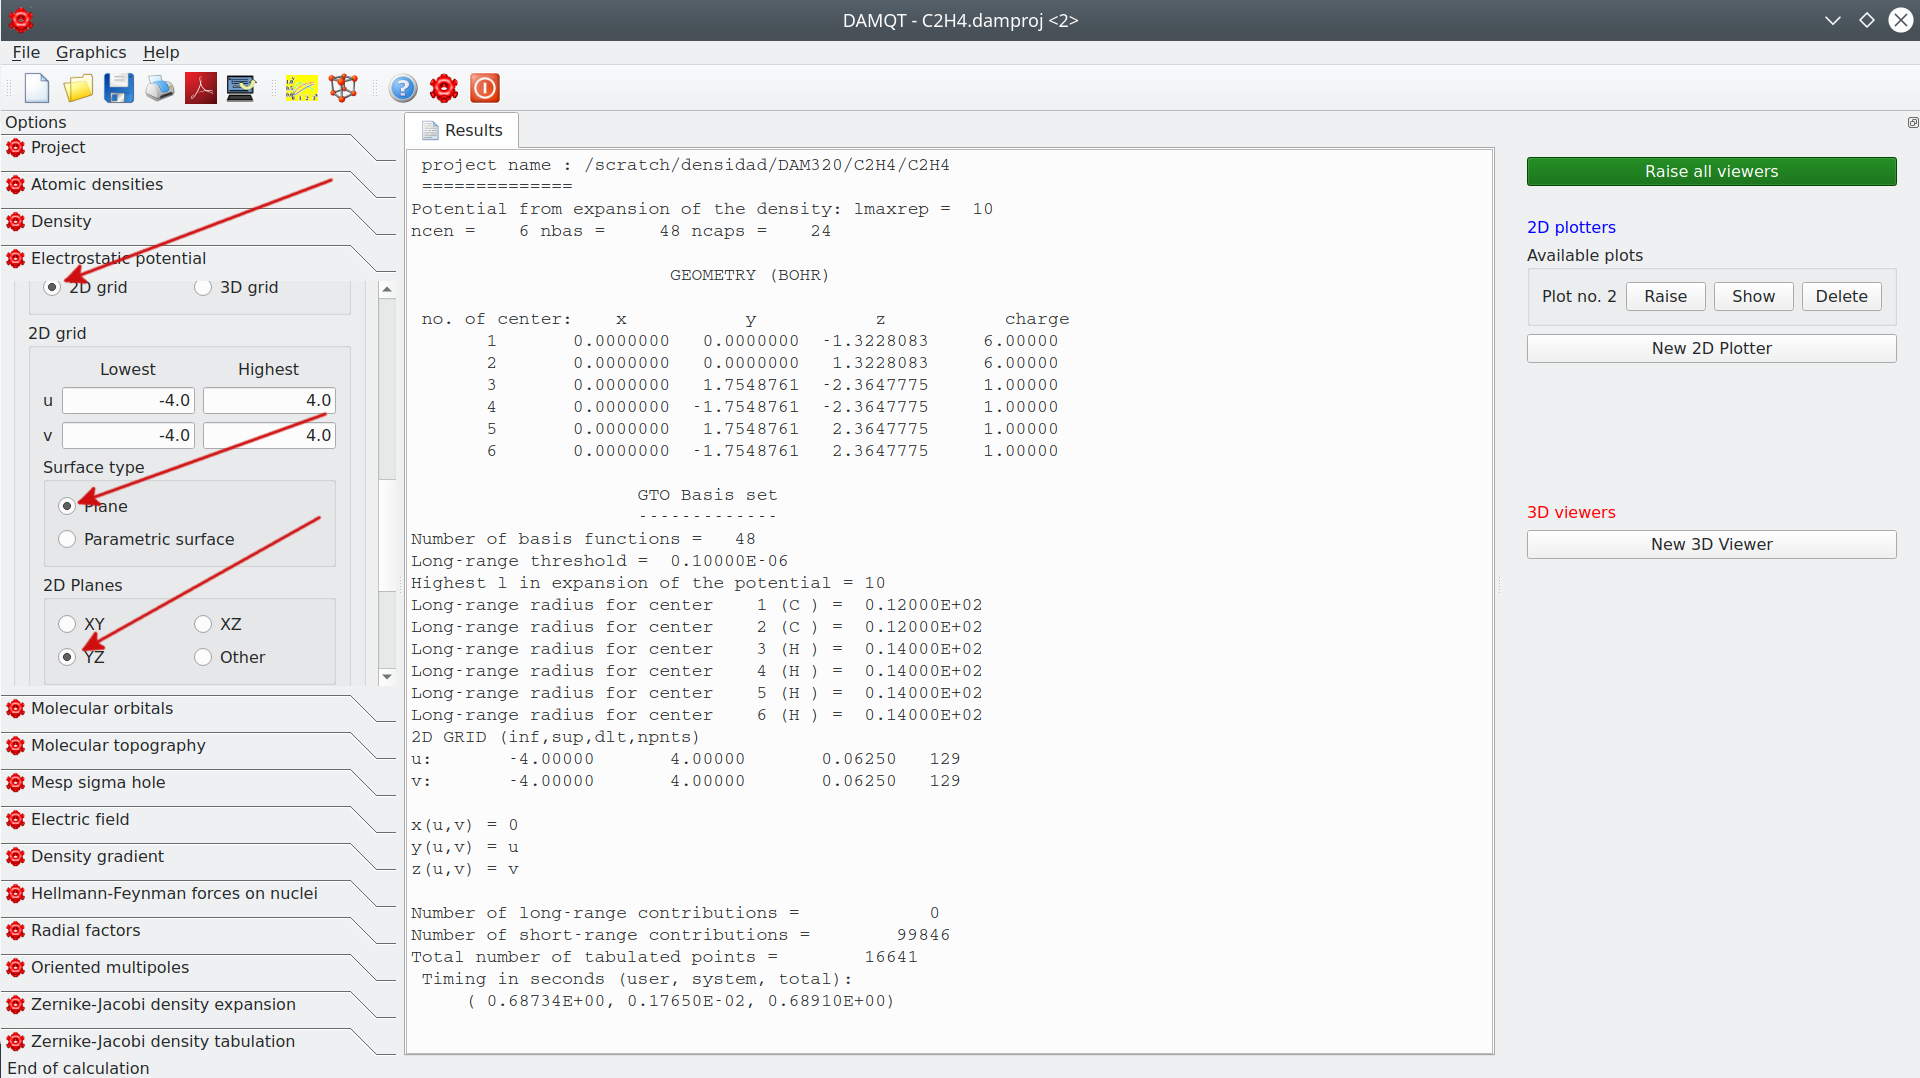
\includegraphics[width=0.95\linewidth]{damqt_QS_fig9.png}
\end{center}
\end{figure} 
\end{minipage}
\begin{minipage}{.5\linewidth}
\begin{figure}[H]
\caption{\label{fig:10}}
\begin{center}
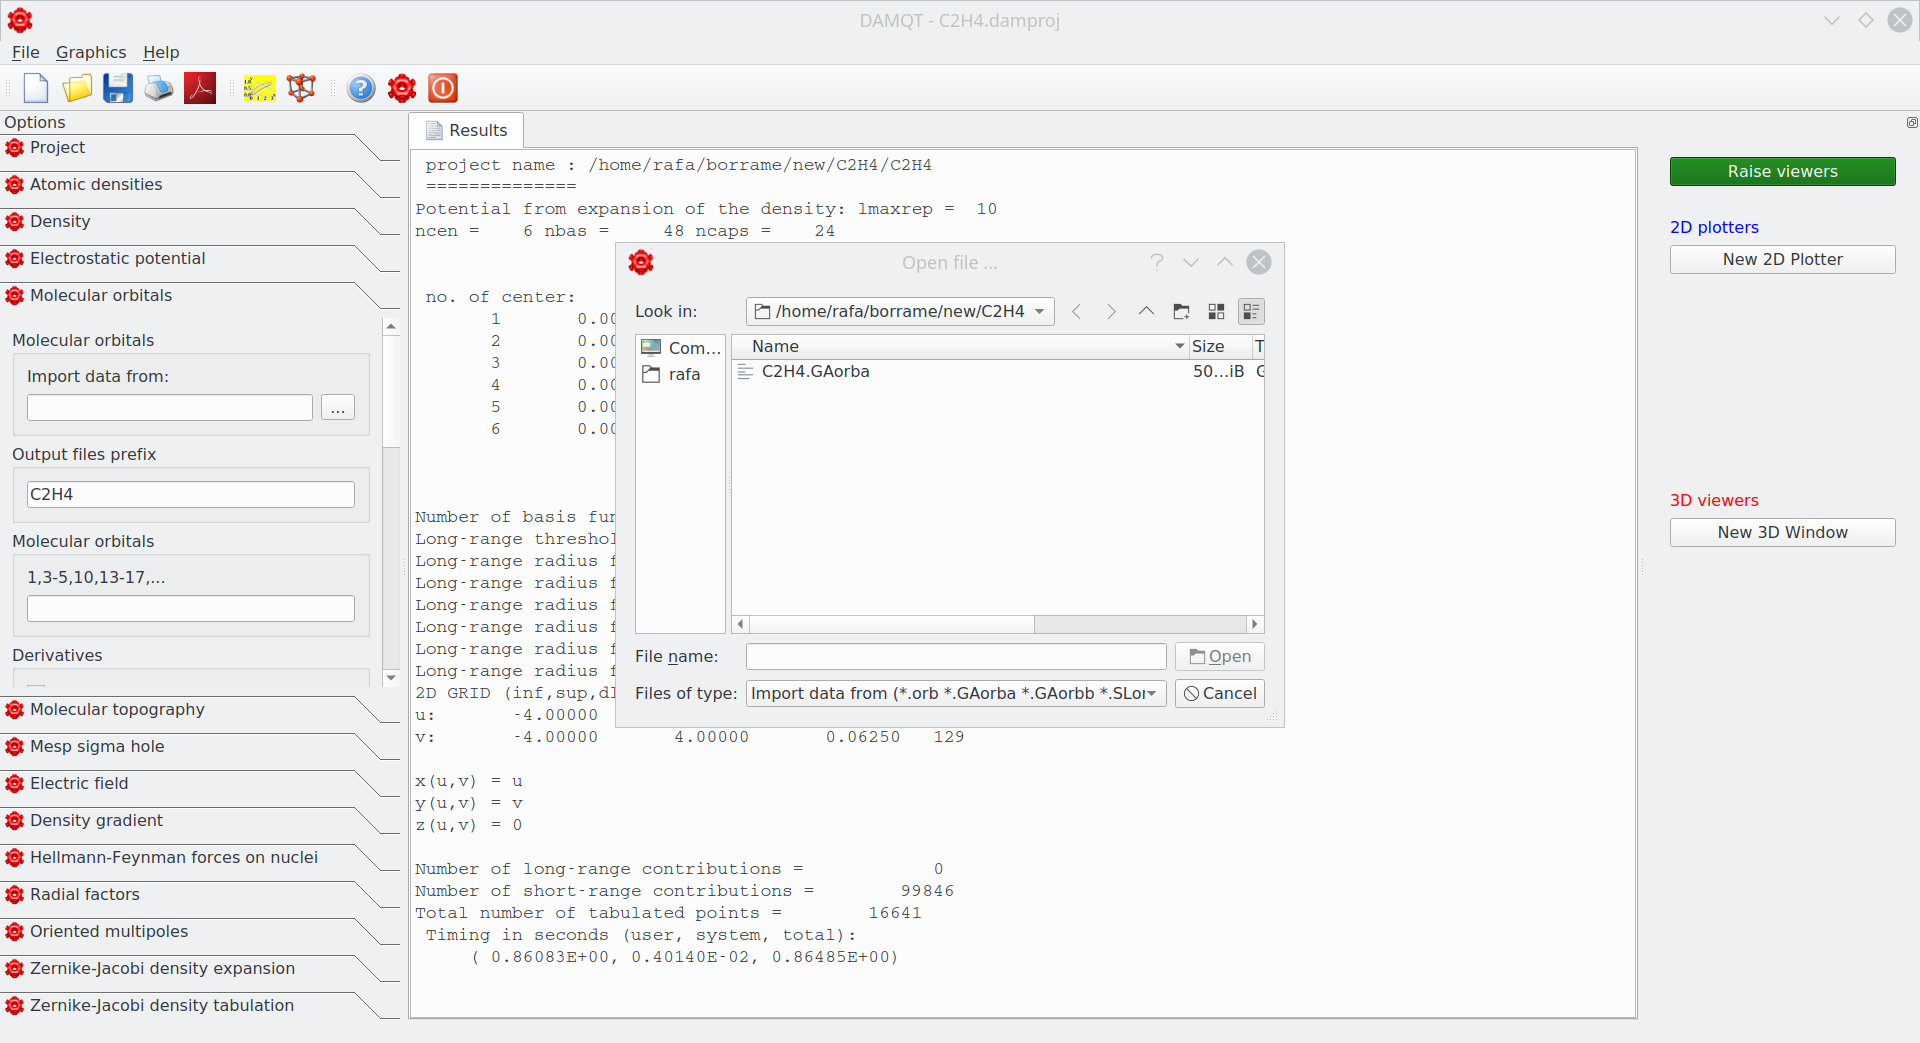
\includegraphics[width=0.95\linewidth]{damqt_QS_fig10.png}
\end{center}
\end{figure} 
\end{minipage}

\begin{minipage}{.5\linewidth}
\begin{figure}[H]
\caption{\label{fig:11}}
\begin{center}
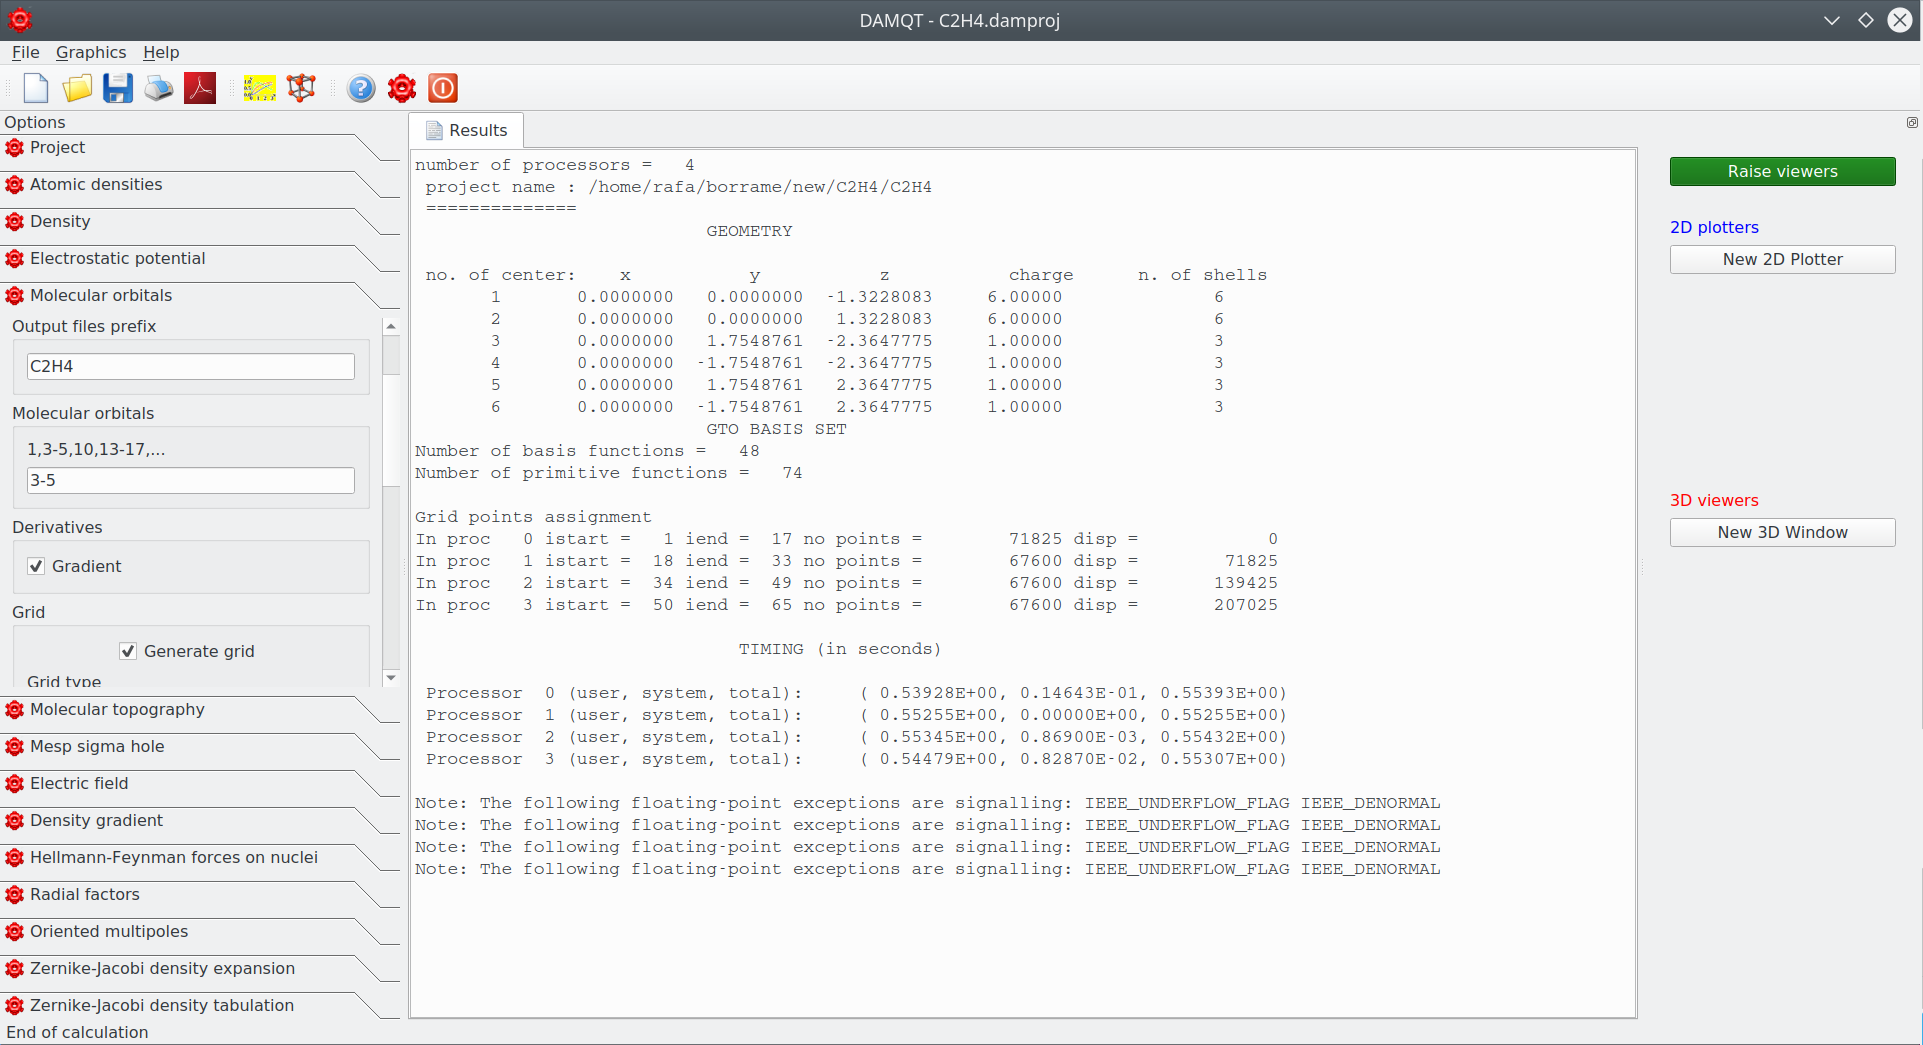
\includegraphics[width=0.95\linewidth]{damqt_QS_fig11.png}
\end{center}
\end{figure} 
\end{minipage}
\begin{minipage}{.5\linewidth}
\begin{figure}[H]
\caption{\label{fig:12}}
\begin{center}
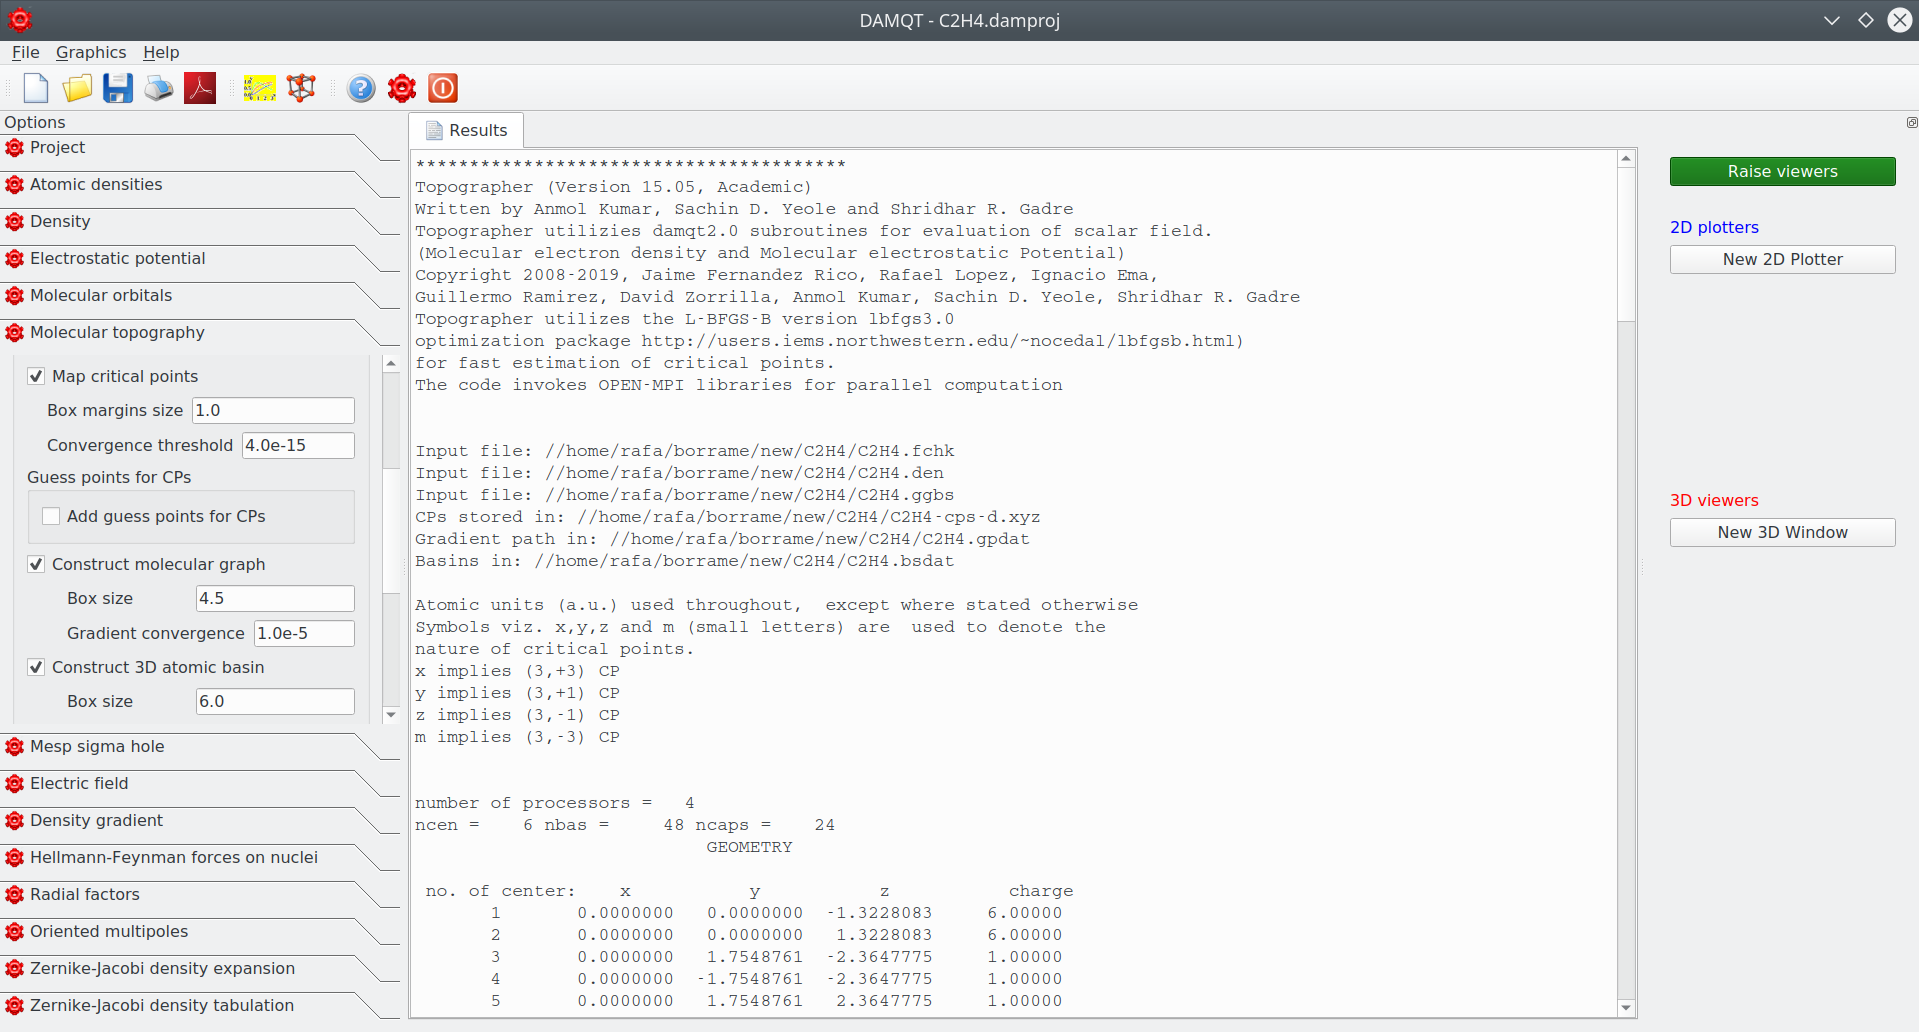
\includegraphics[width=0.95\linewidth]{damqt_QS_fig12.png}
\end{center}
\end{figure} 
\end{minipage}

\begin{minipage}{.5\linewidth}
\begin{figure}[H]
\caption{\label{fig:13}}
\begin{center}
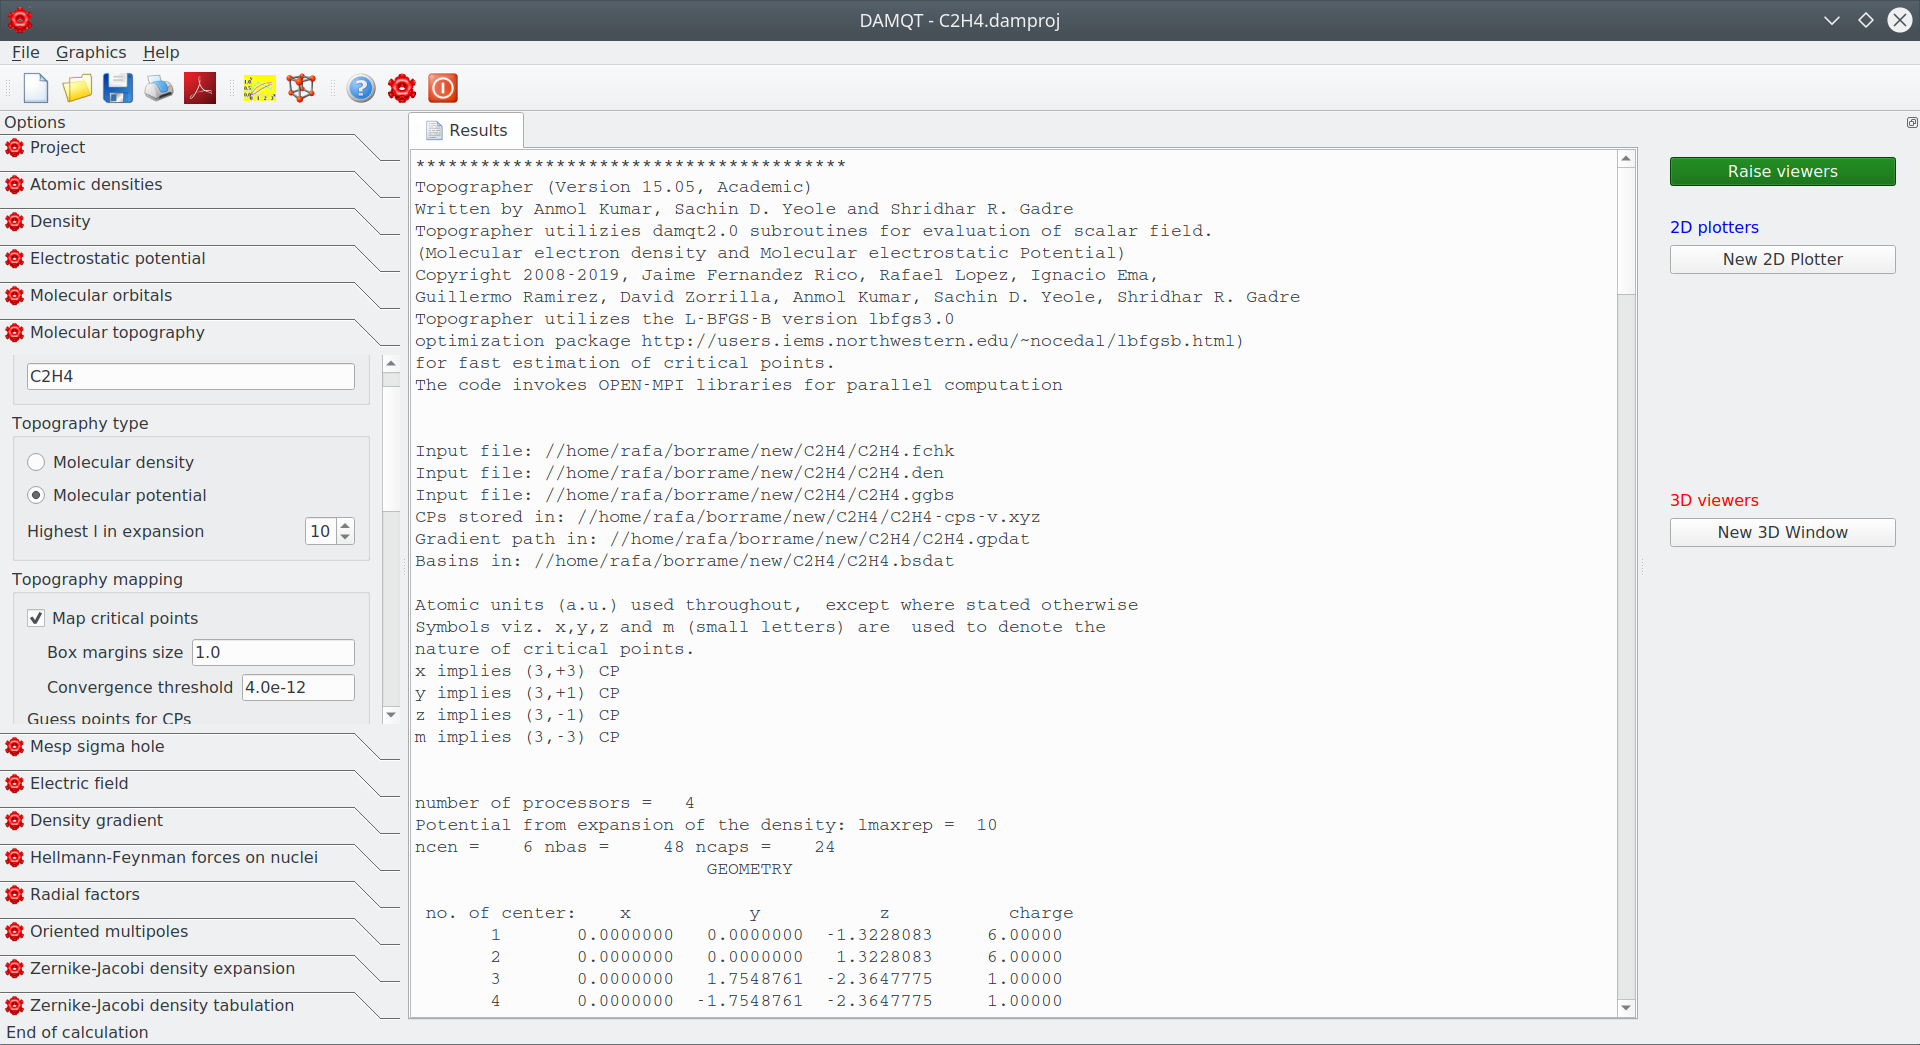
\includegraphics[width=0.95\linewidth]{damqt_QS_fig13.png}
\end{center}
\end{figure} 
\end{minipage}
\begin{minipage}{.5\linewidth}
\begin{figure}[H]
\caption{\label{fig:14}}
\begin{center}
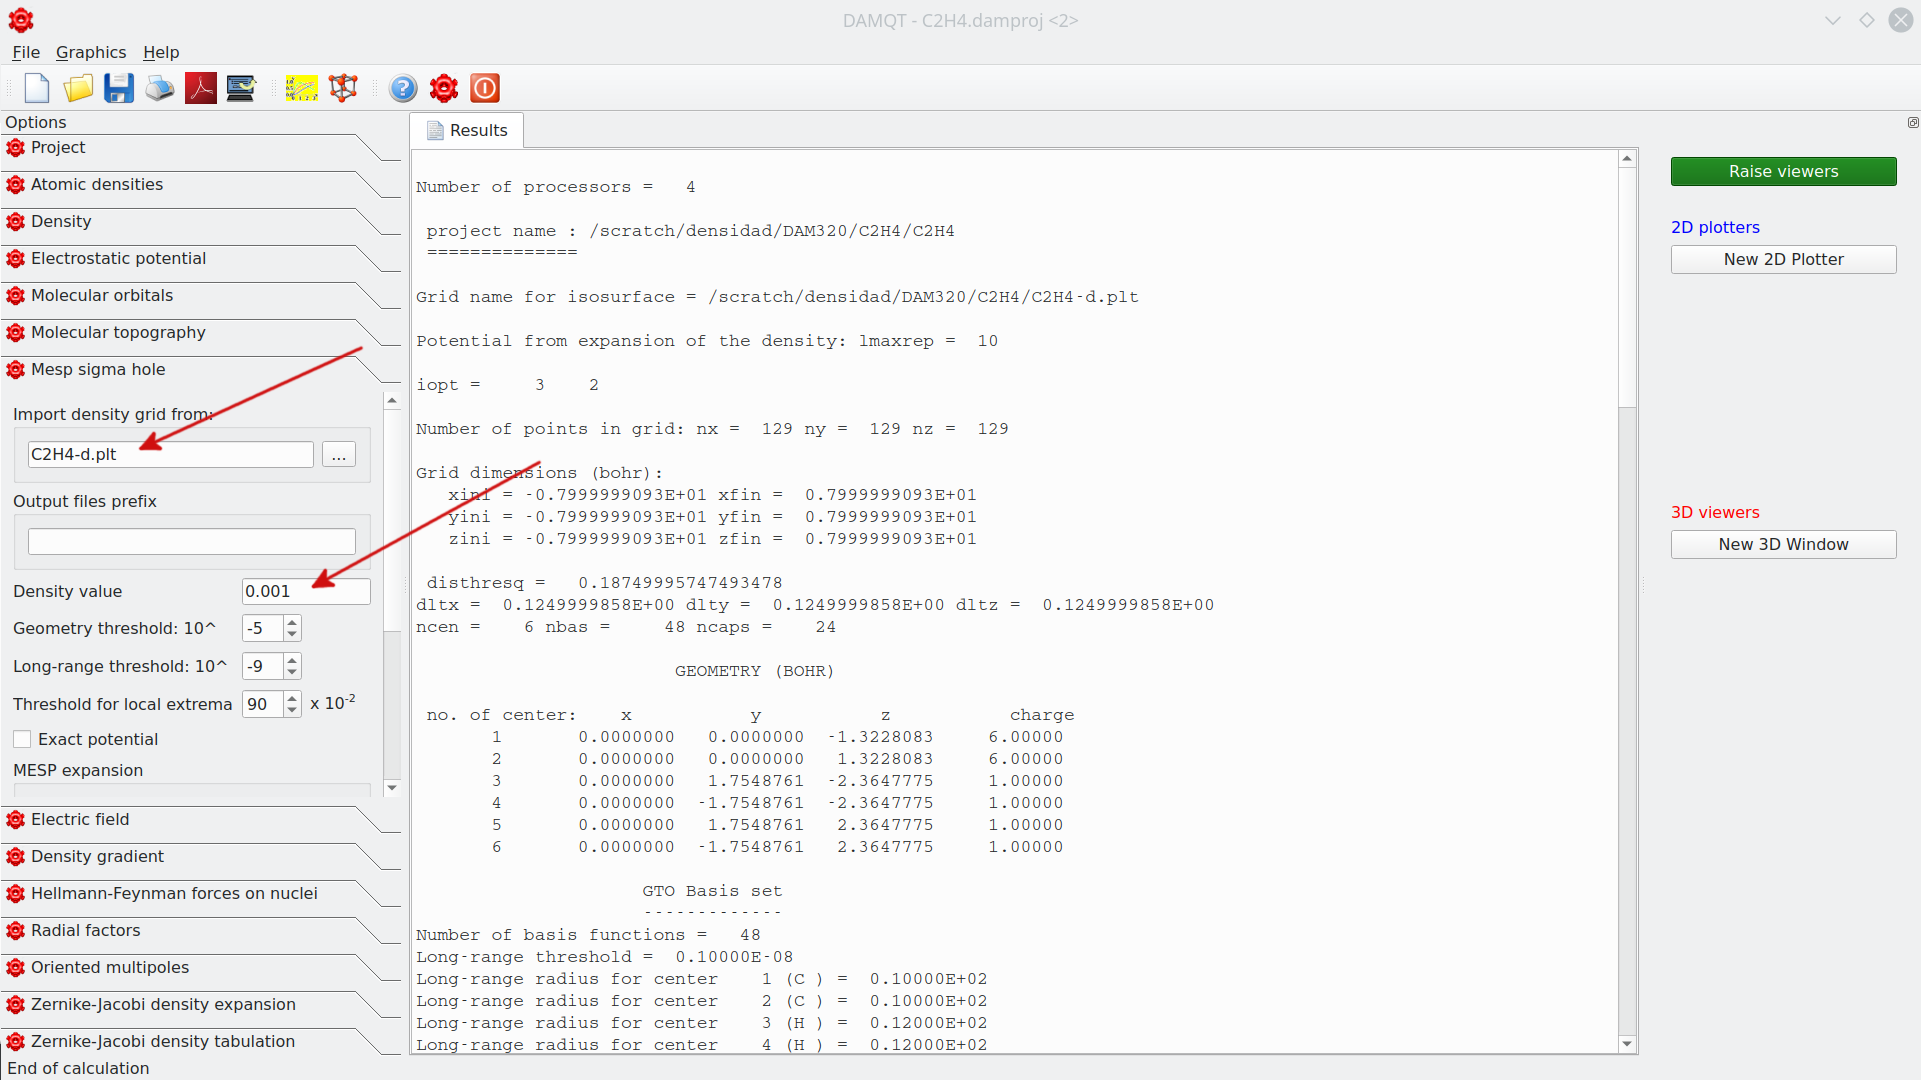
\includegraphics[width=0.95\linewidth]{damqt_QS_fig14.png}
\end{center}
\end{figure} 
\end{minipage}

\begin{minipage}{.5\linewidth}
\begin{figure}[H]
\caption{\label{fig:15}}
\begin{center}
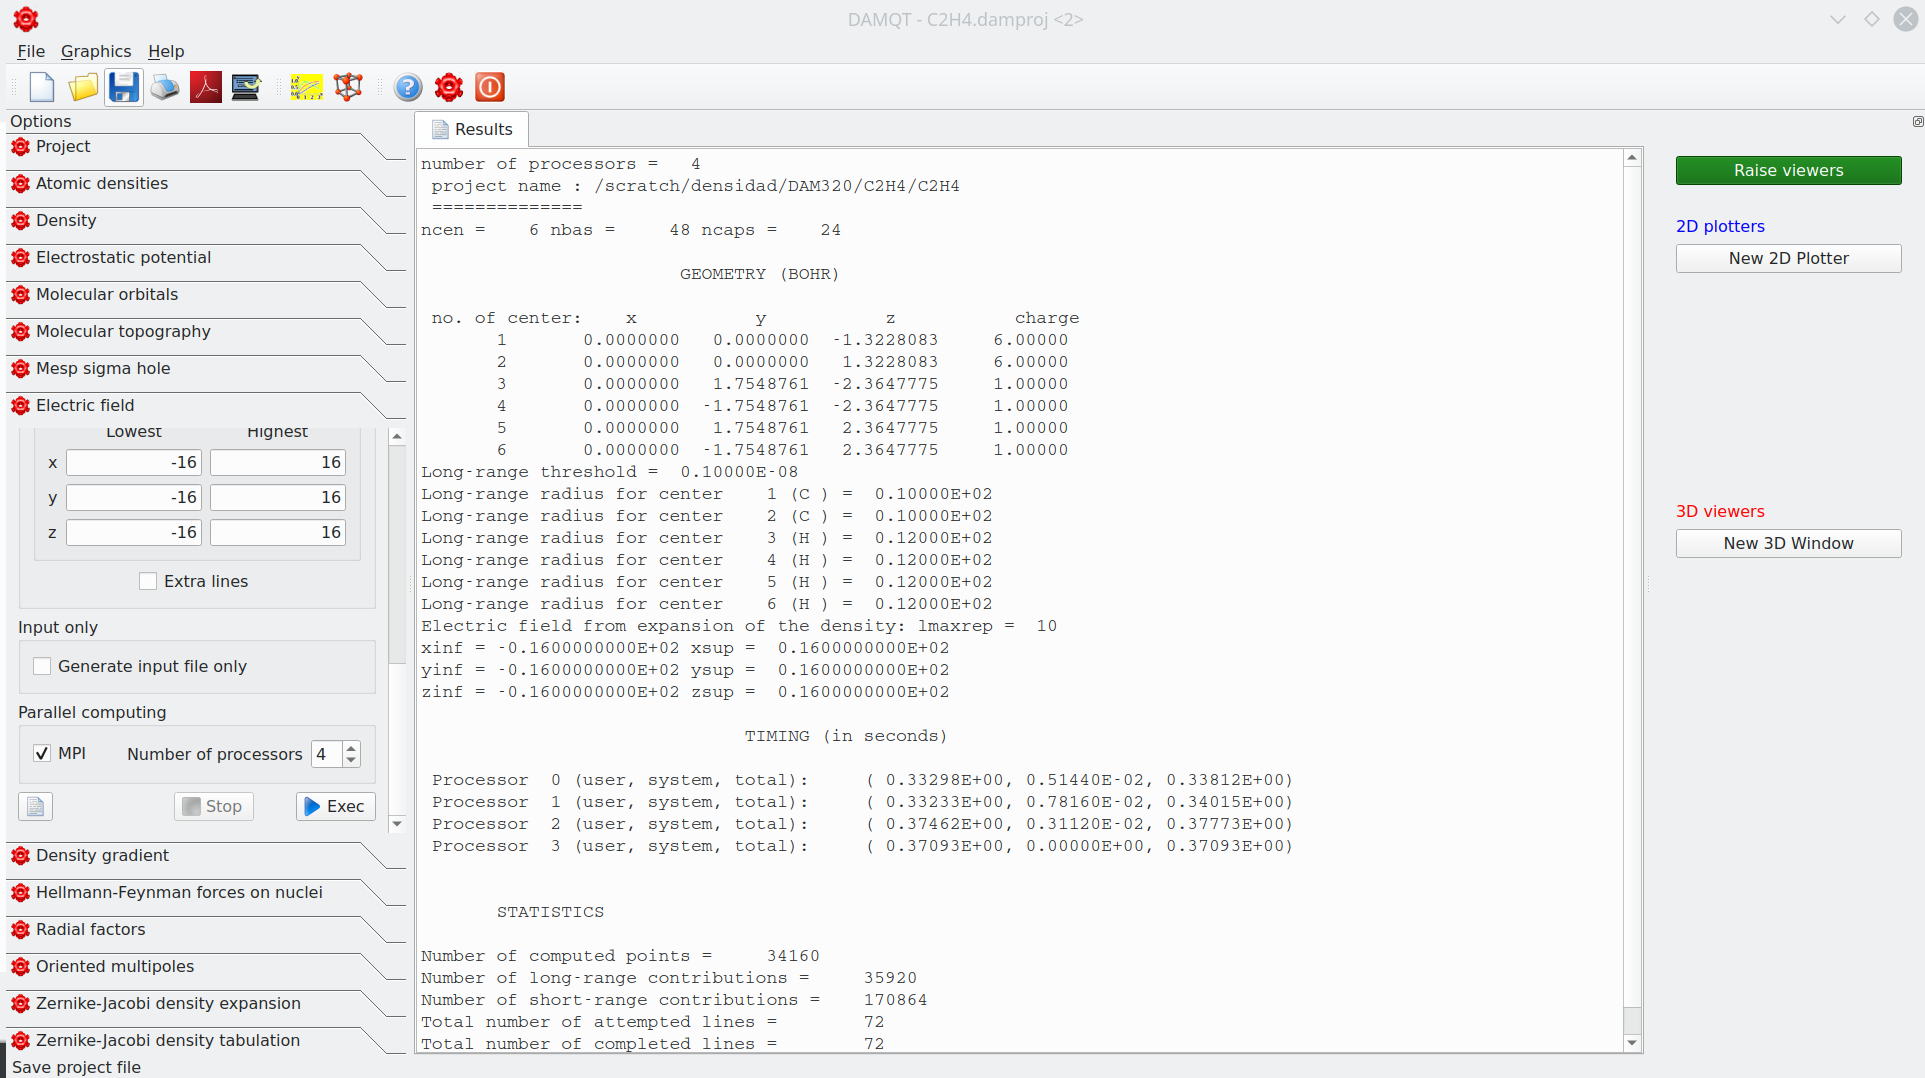
\includegraphics[width=0.95\linewidth]{damqt_QS_fig15.png}
\end{center}
\end{figure} 
\end{minipage}
\begin{minipage}{.5\linewidth}
\begin{figure}[H]
\caption{\label{fig:16}}
\begin{center}
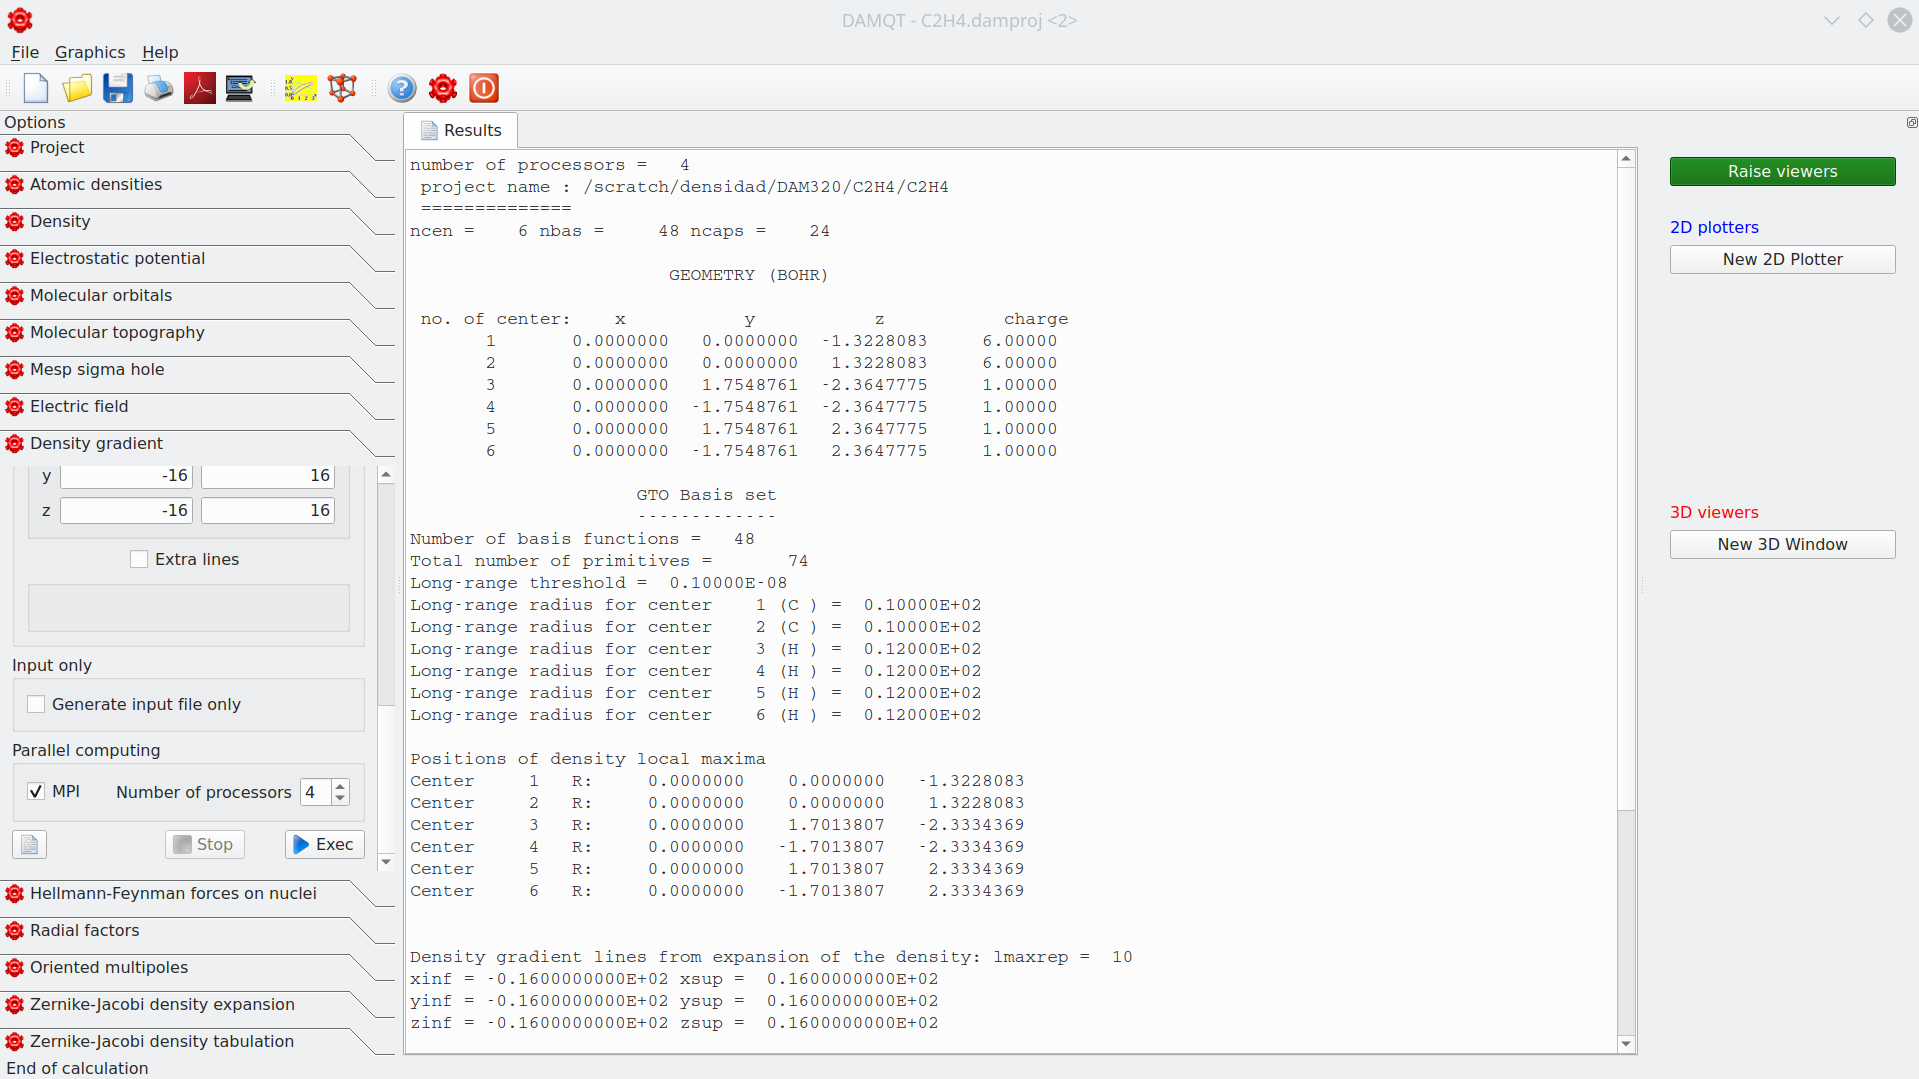
\includegraphics[width=0.95\linewidth]{damqt_QS_fig16.png}
\end{center}
\end{figure} 
\end{minipage}

\begin{minipage}{.5\linewidth}
\begin{figure}[H]
\caption{\label{fig:17}}
\begin{center}
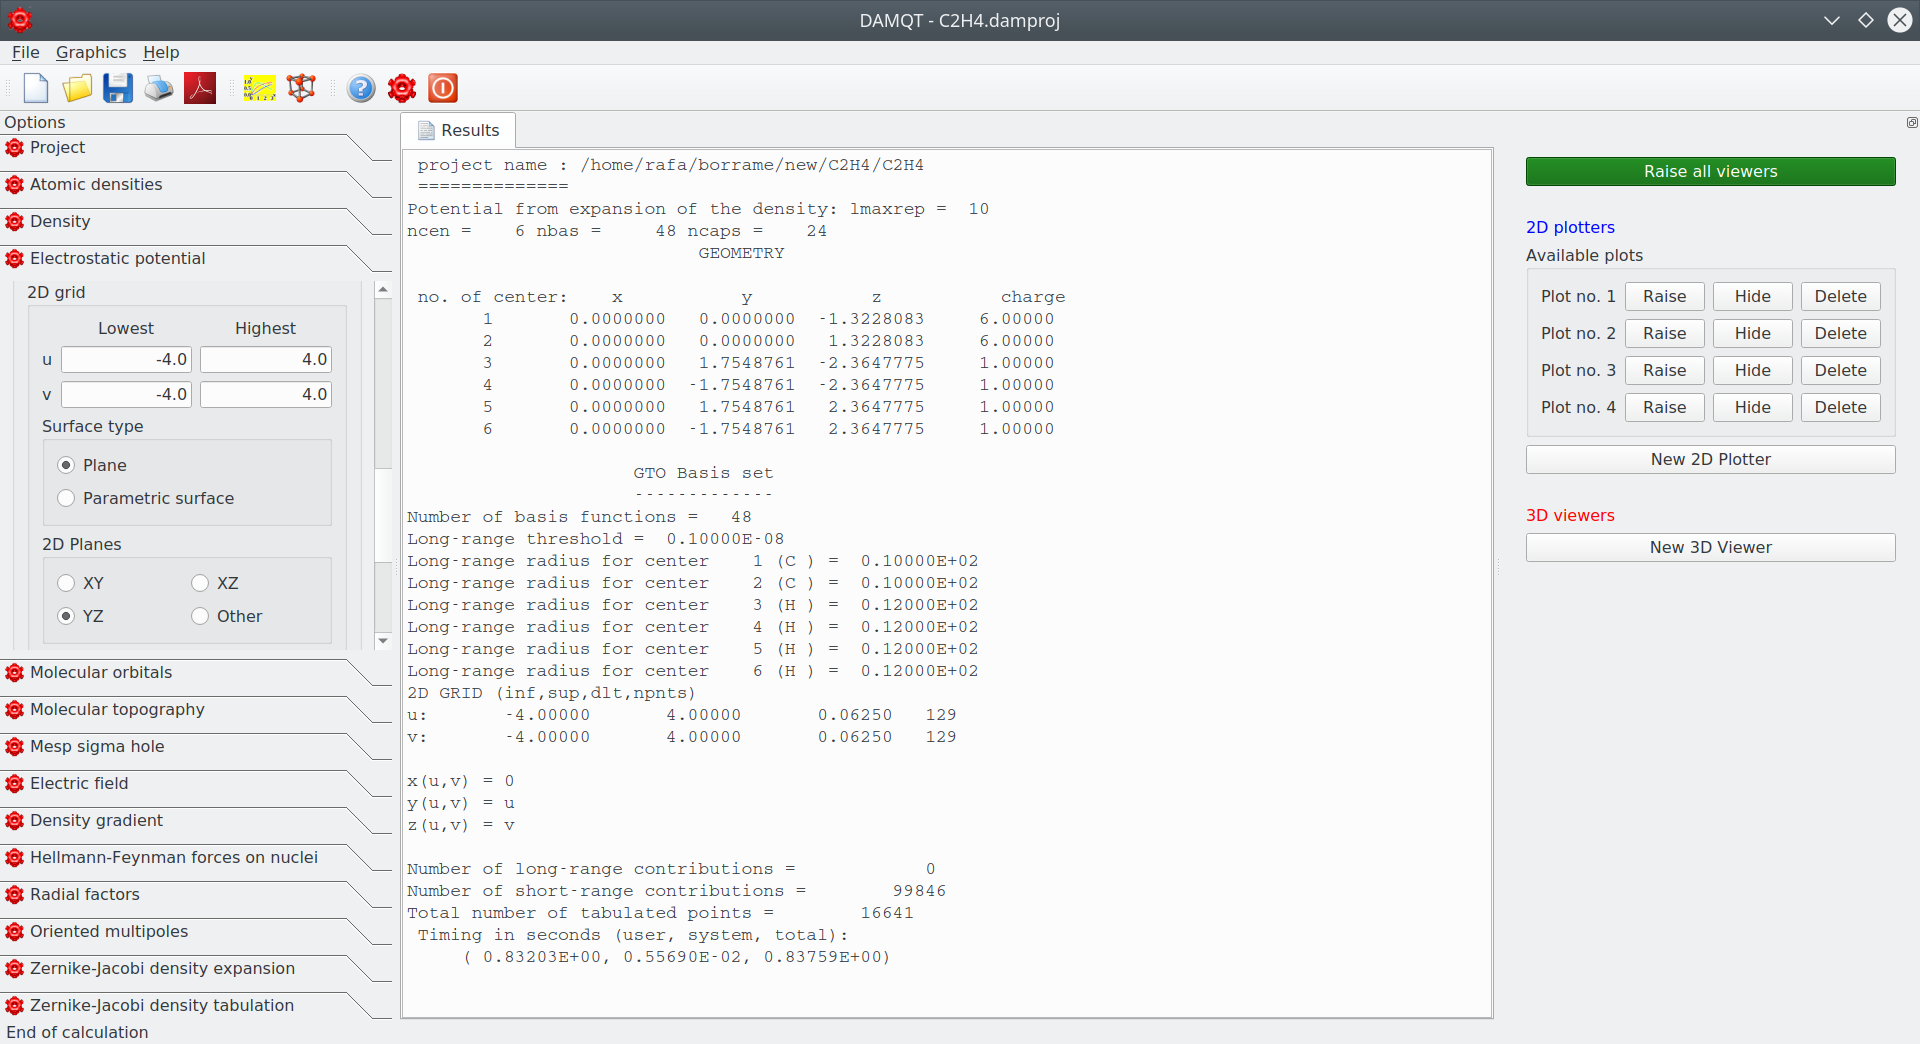
\includegraphics[width=0.95\linewidth]{damqt_QS_fig17.png}
\end{center}
\end{figure} 
\end{minipage}
\begin{minipage}{.5\linewidth}
\begin{figure}[H]
\caption{\label{fig:18}}
\begin{center}
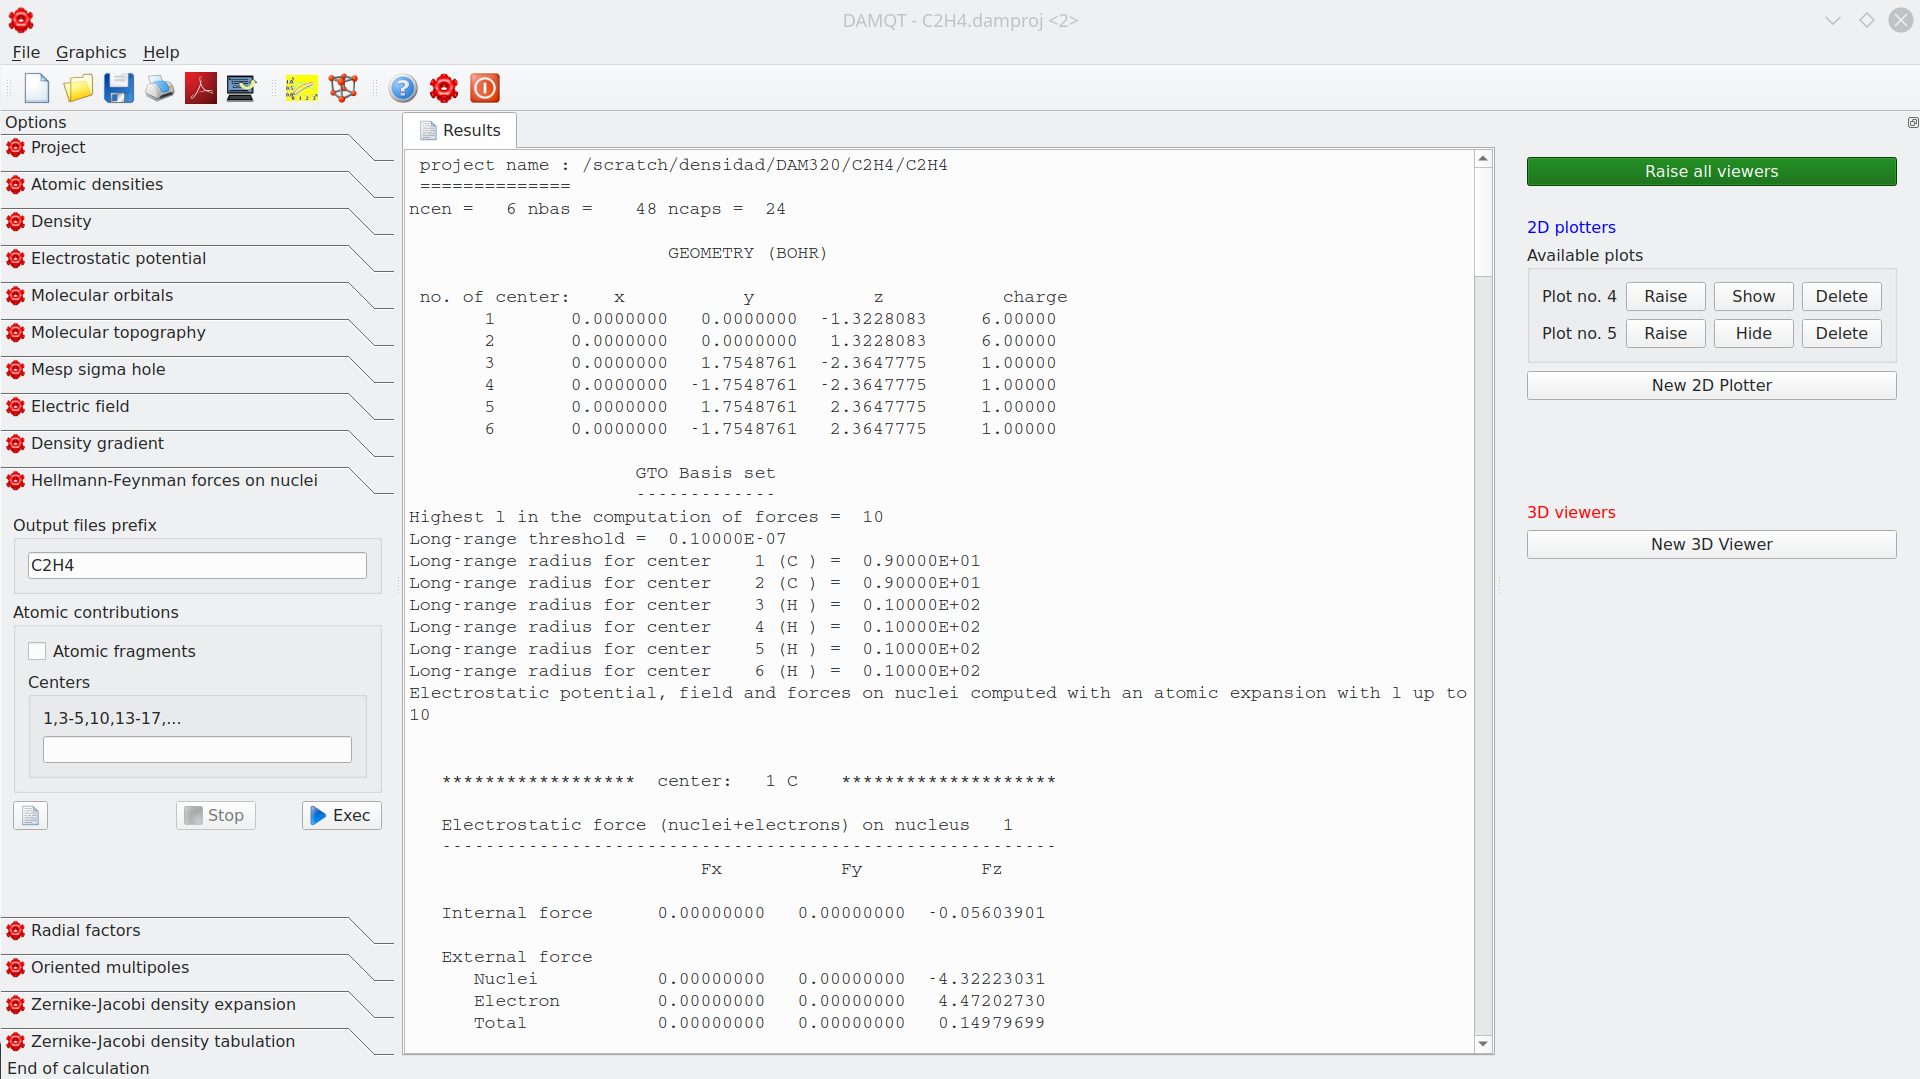
\includegraphics[width=0.95\linewidth]{damqt_QS_fig18.png}
\end{center}
\end{figure} 
\end{minipage}

\begin{minipage}{.5\linewidth}
\begin{figure}[H]
\caption{\label{fig:19}}
\begin{center}
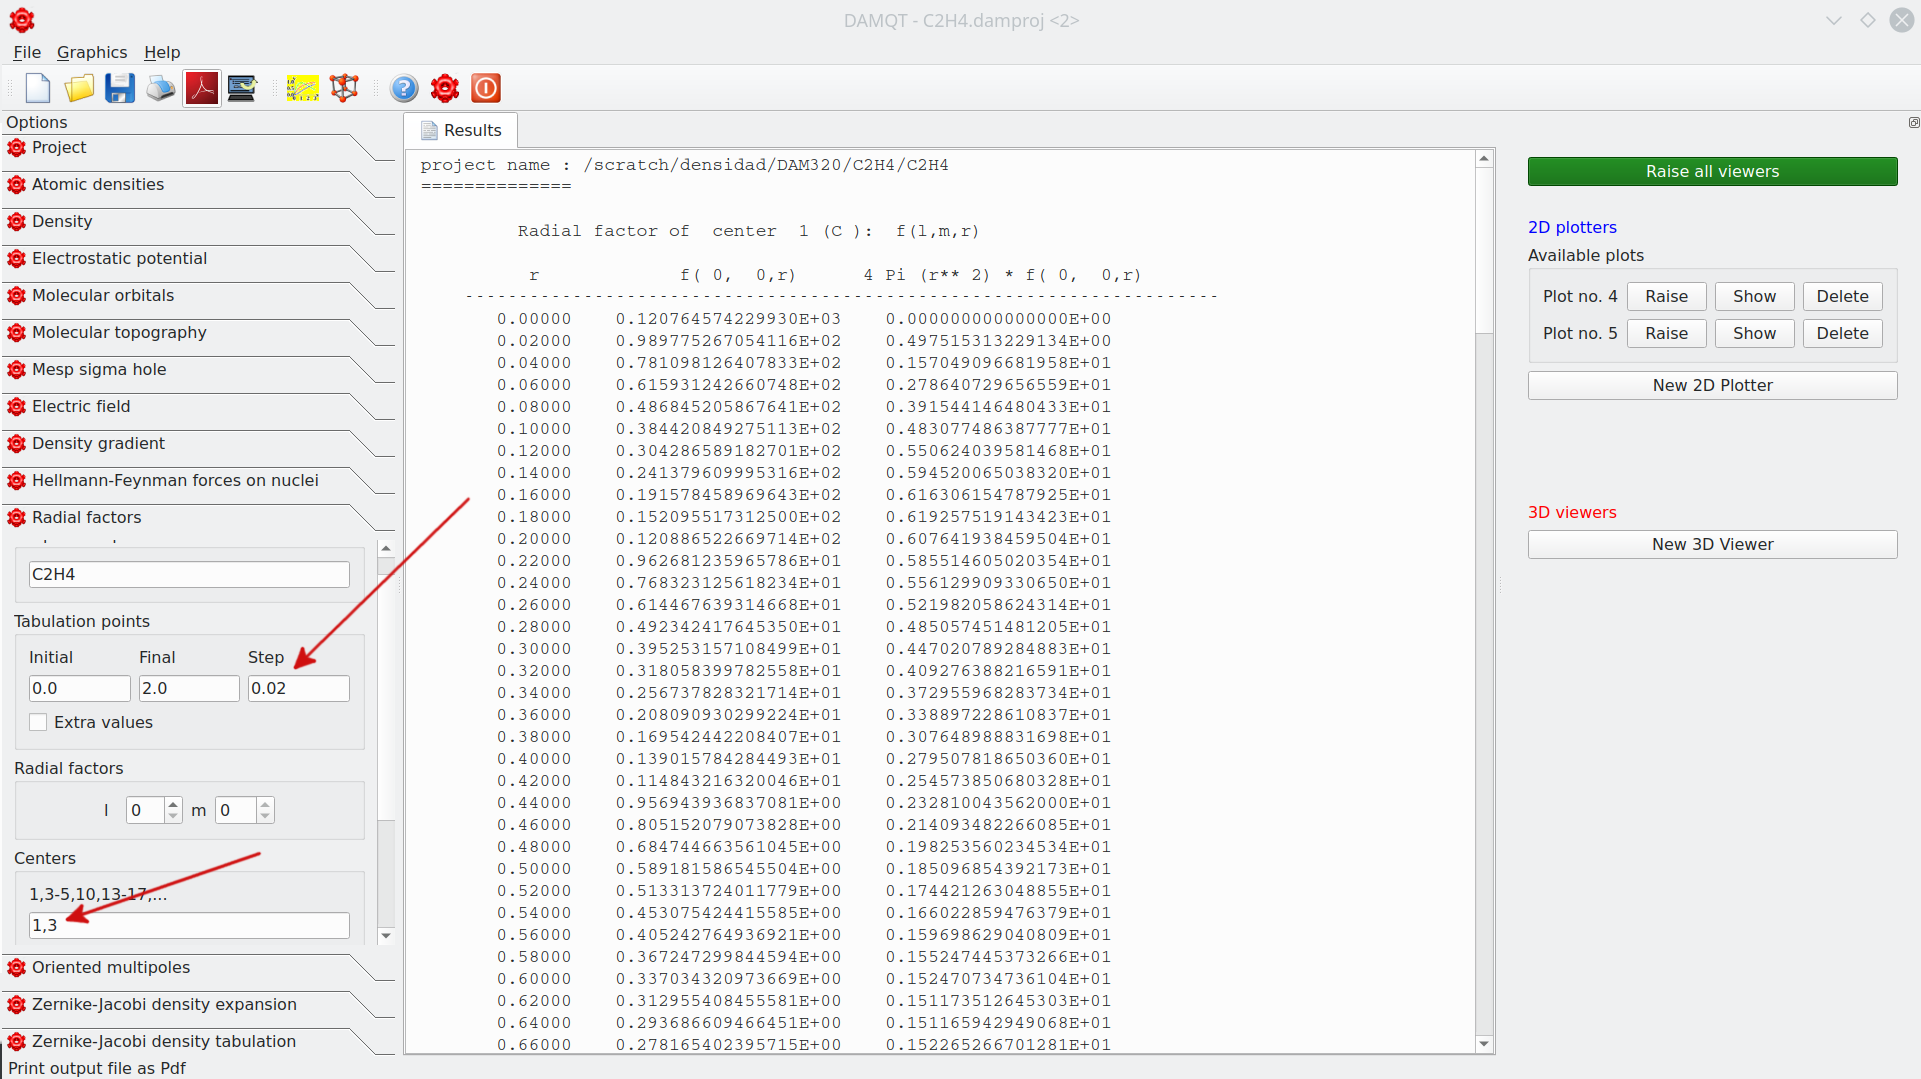
\includegraphics[width=0.95\linewidth]{damqt_QS_fig19.png}
\end{center}
\end{figure} 
\end{minipage}
\begin{minipage}{.5\linewidth}
\begin{figure}[H]
\caption{\label{fig:20}}
\begin{center}
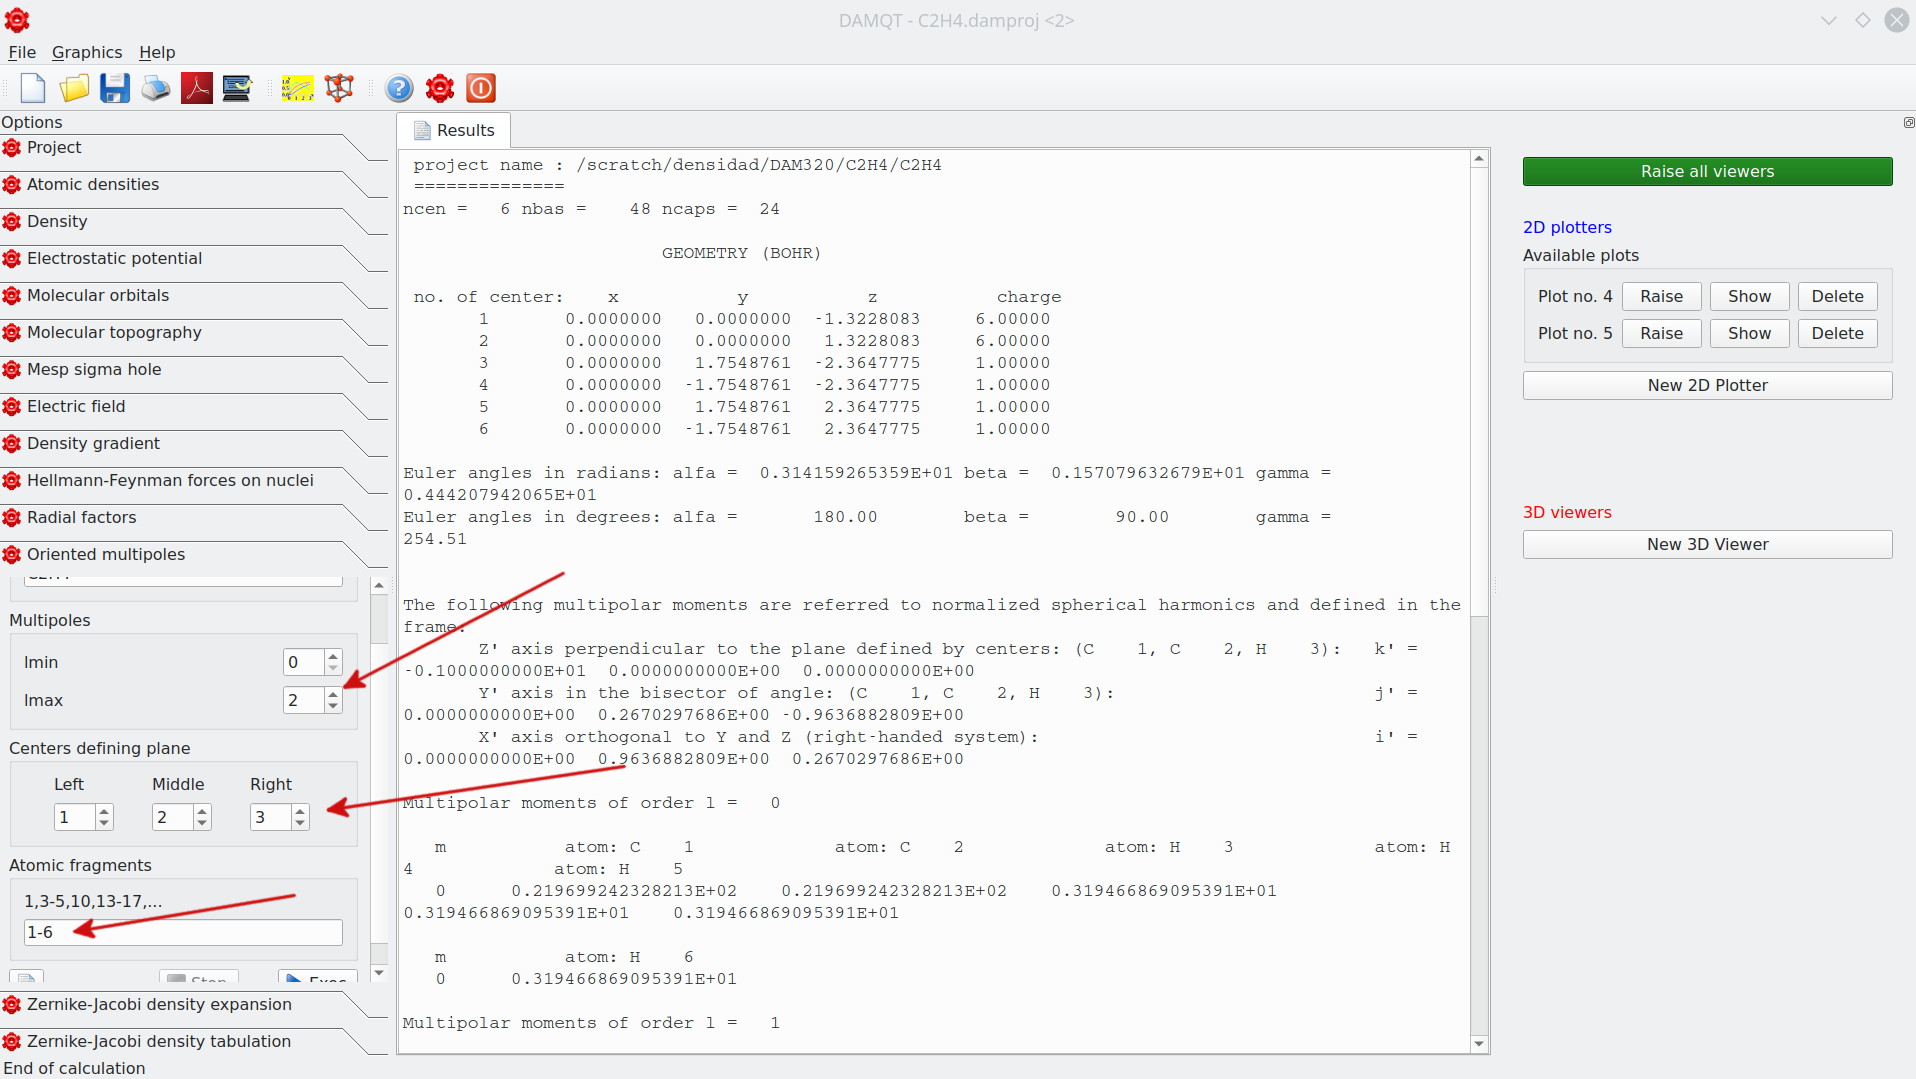
\includegraphics[width=0.95\linewidth]{damqt_QS_fig20.png}
\end{center}
\end{figure} 
\end{minipage}

\begin{minipage}{.5\linewidth}
\begin{figure}[H]
\caption{\label{fig:21}}
\begin{center}
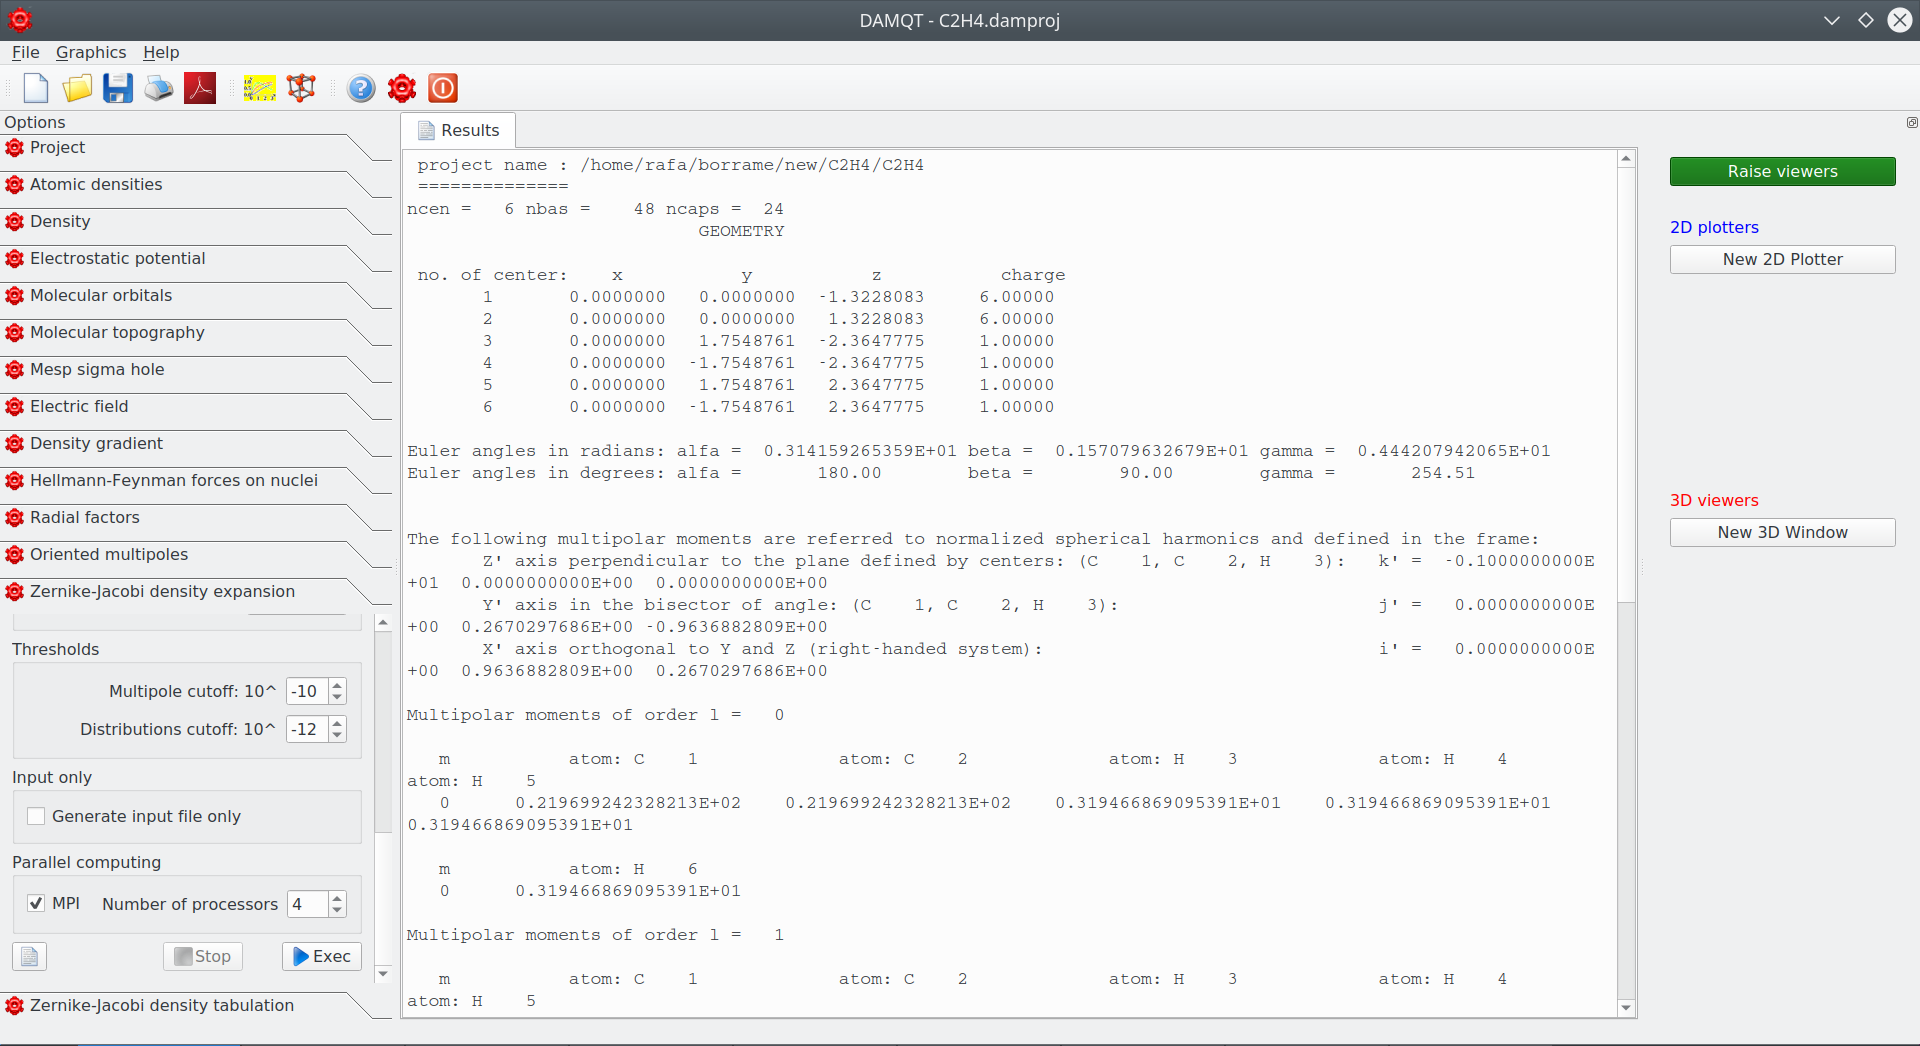
\includegraphics[width=0.95\linewidth]{damqt_QS_fig21.png}
\end{center}
\end{figure} 
\end{minipage}
\begin{minipage}{.5\linewidth}
\begin{figure}[H]
\caption{\label{fig:22}}
\begin{center}
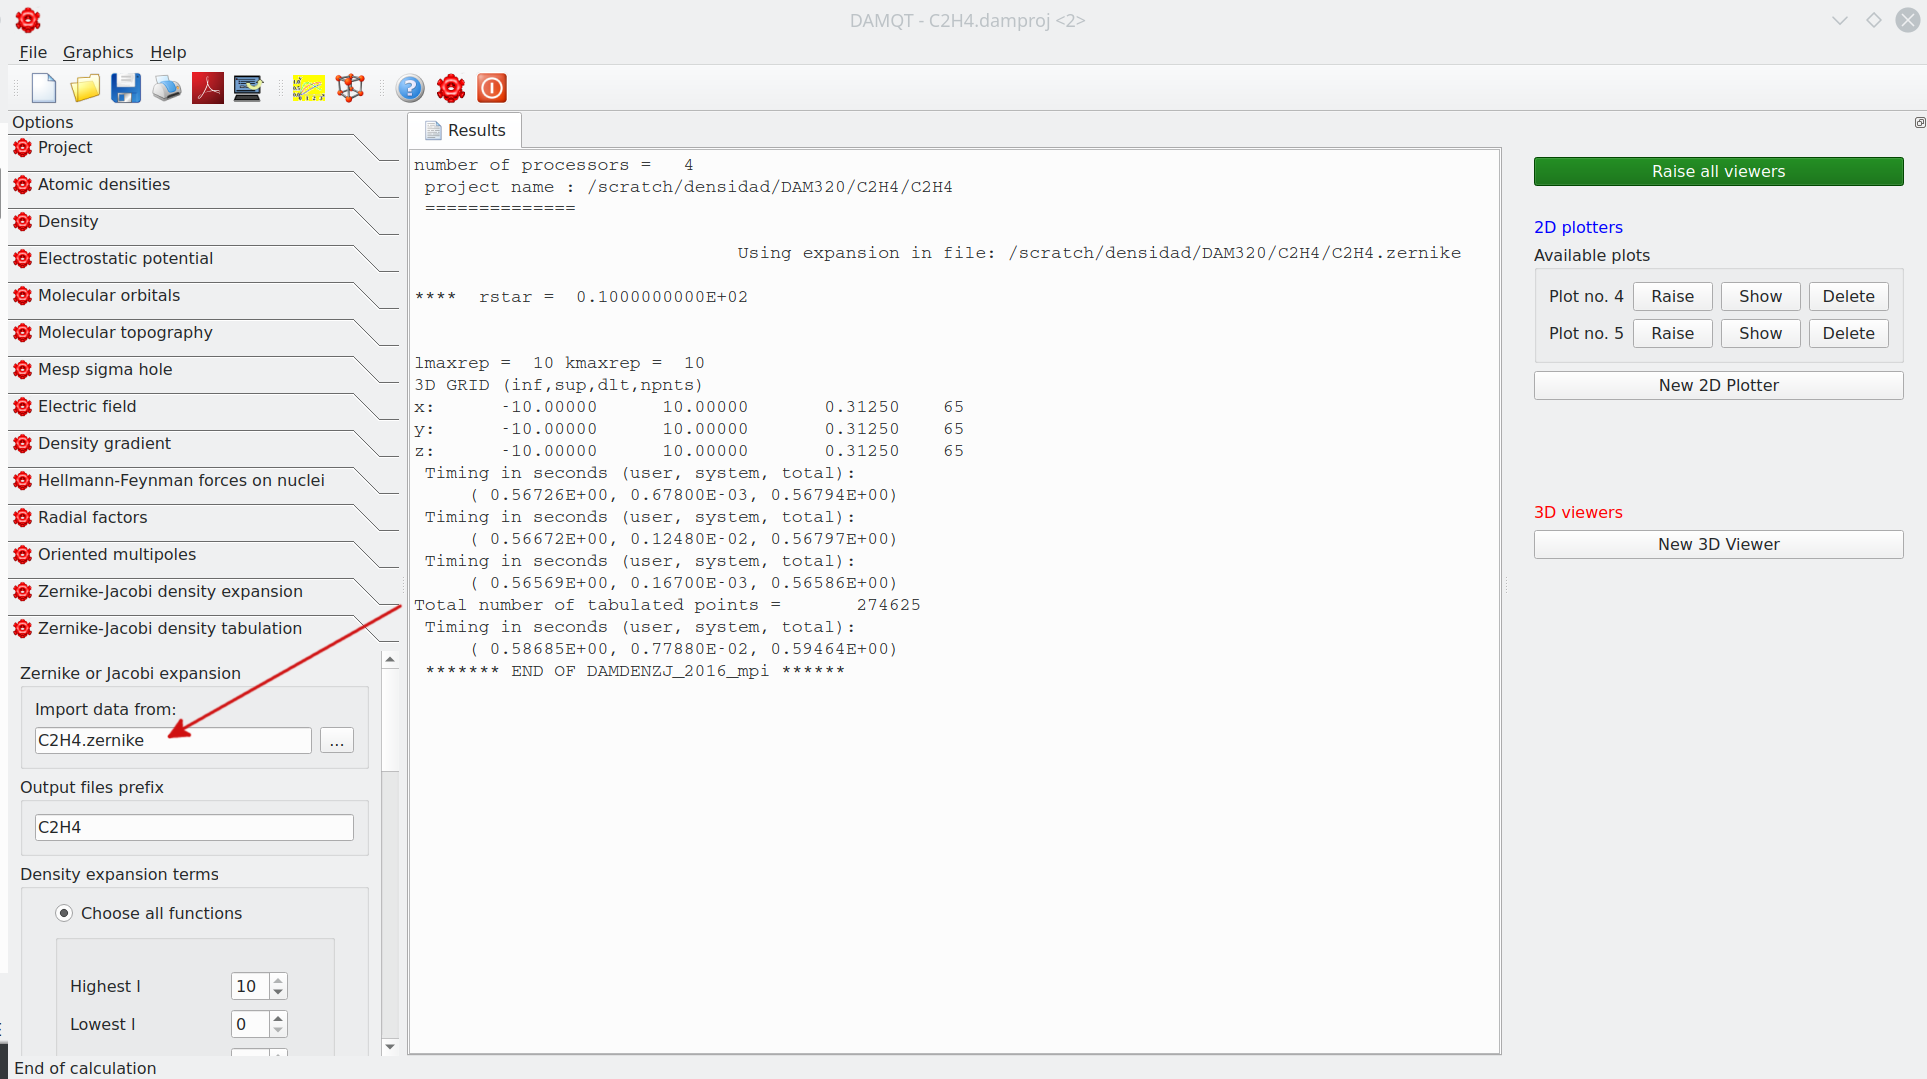
\includegraphics[width=0.95\linewidth]{damqt_QS_fig22.png}
\end{center}
\end{figure} 
\end{minipage}

\begin{minipage}{.5\linewidth}
\begin{figure}[H]
\caption{\label{fig:23}}
\begin{center}
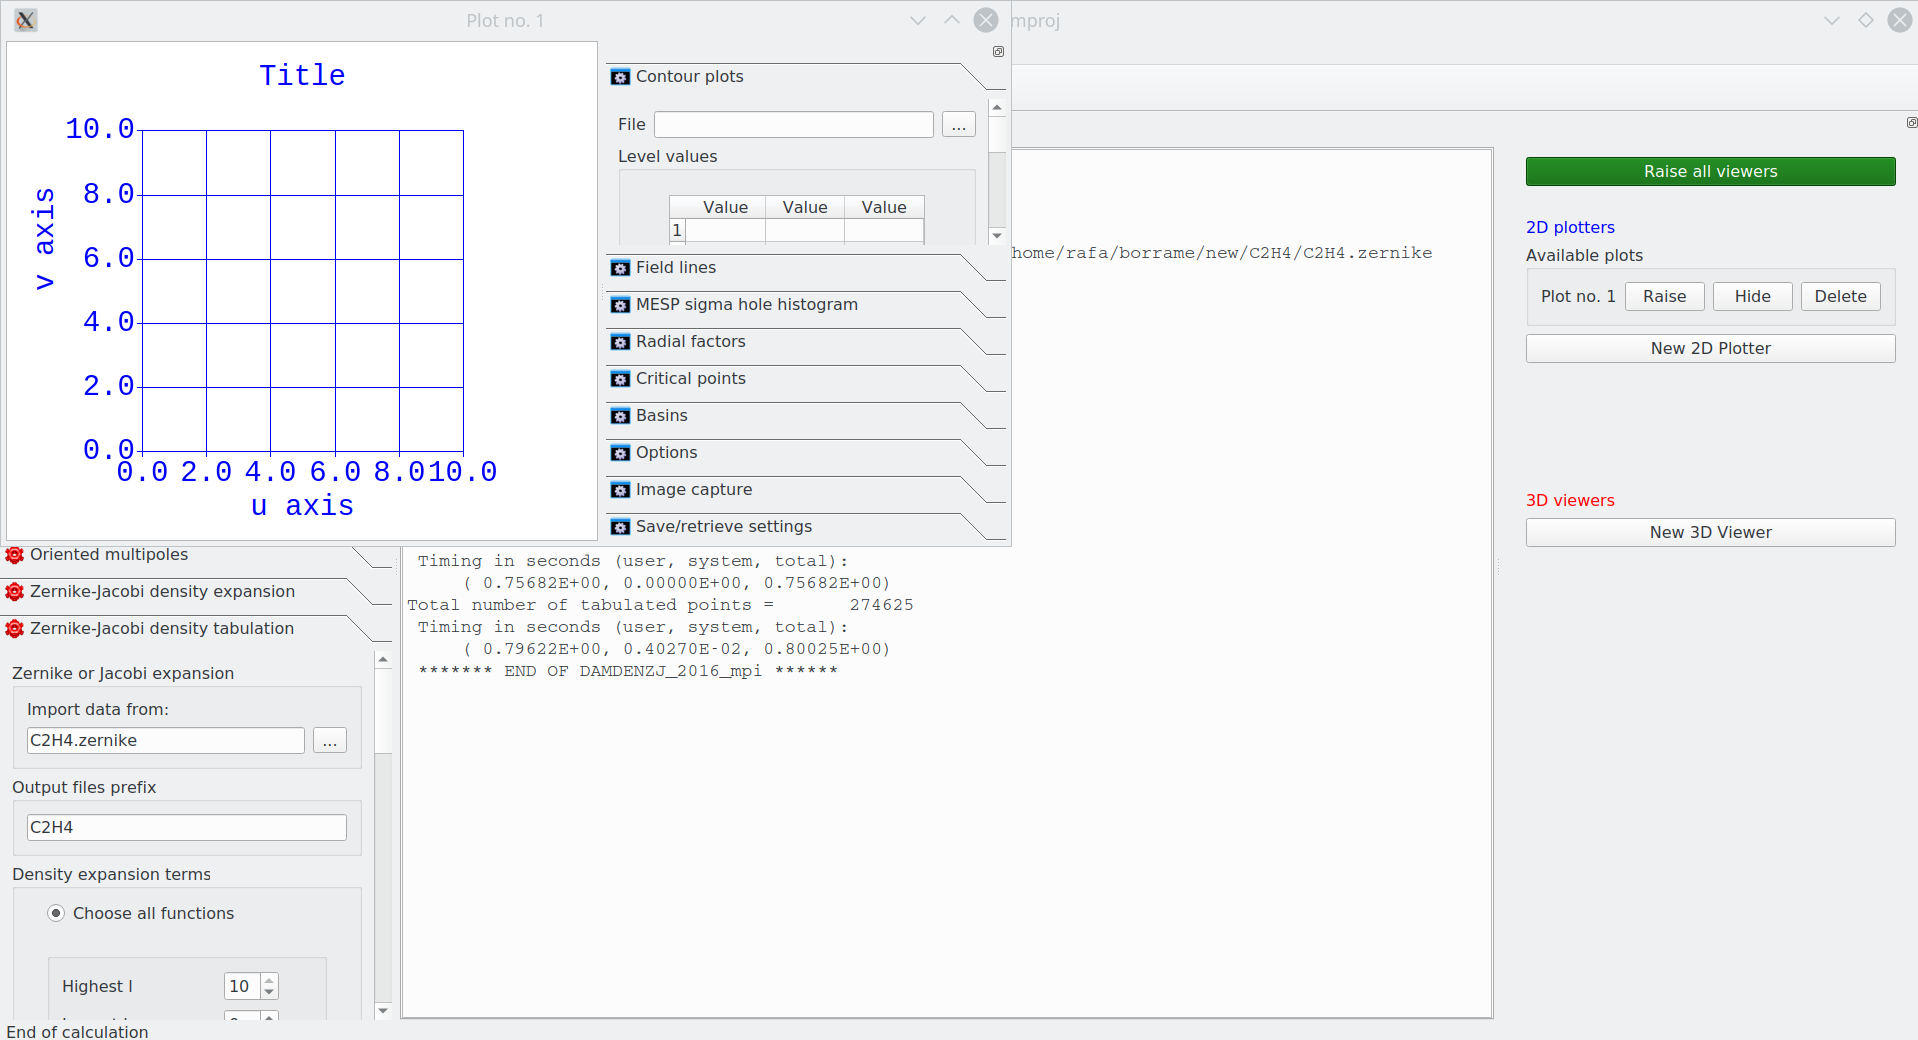
\includegraphics[width=0.95\linewidth]{damqt_QS_fig23.png}
\end{center}
\end{figure} 
\end{minipage}
\begin{minipage}{.5\linewidth}
\begin{figure}[H]
\caption{\label{fig:24}}
\begin{center}
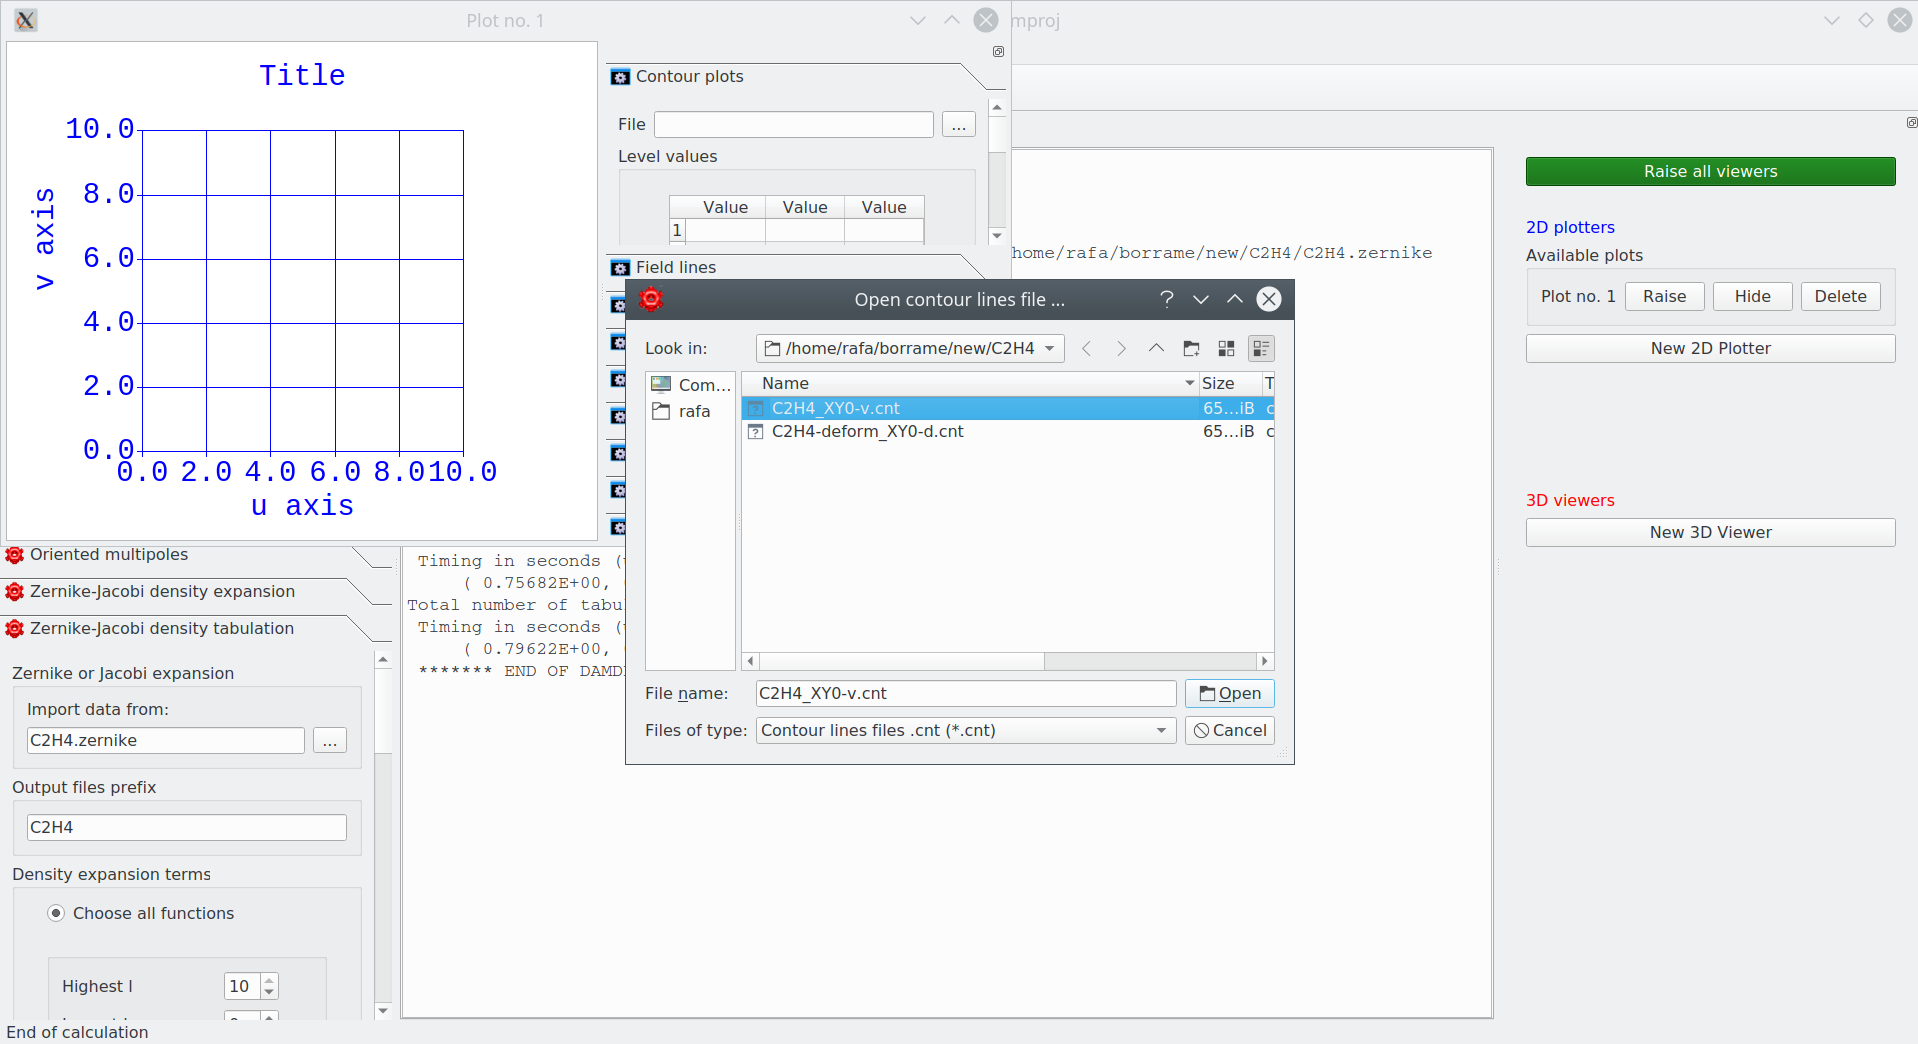
\includegraphics[width=0.95\linewidth]{damqt_QS_fig24.png}
\end{center}
\end{figure} 
\end{minipage}

\begin{minipage}{.5\linewidth}
\begin{figure}[H]
\caption{\label{fig:25}}
\begin{center}
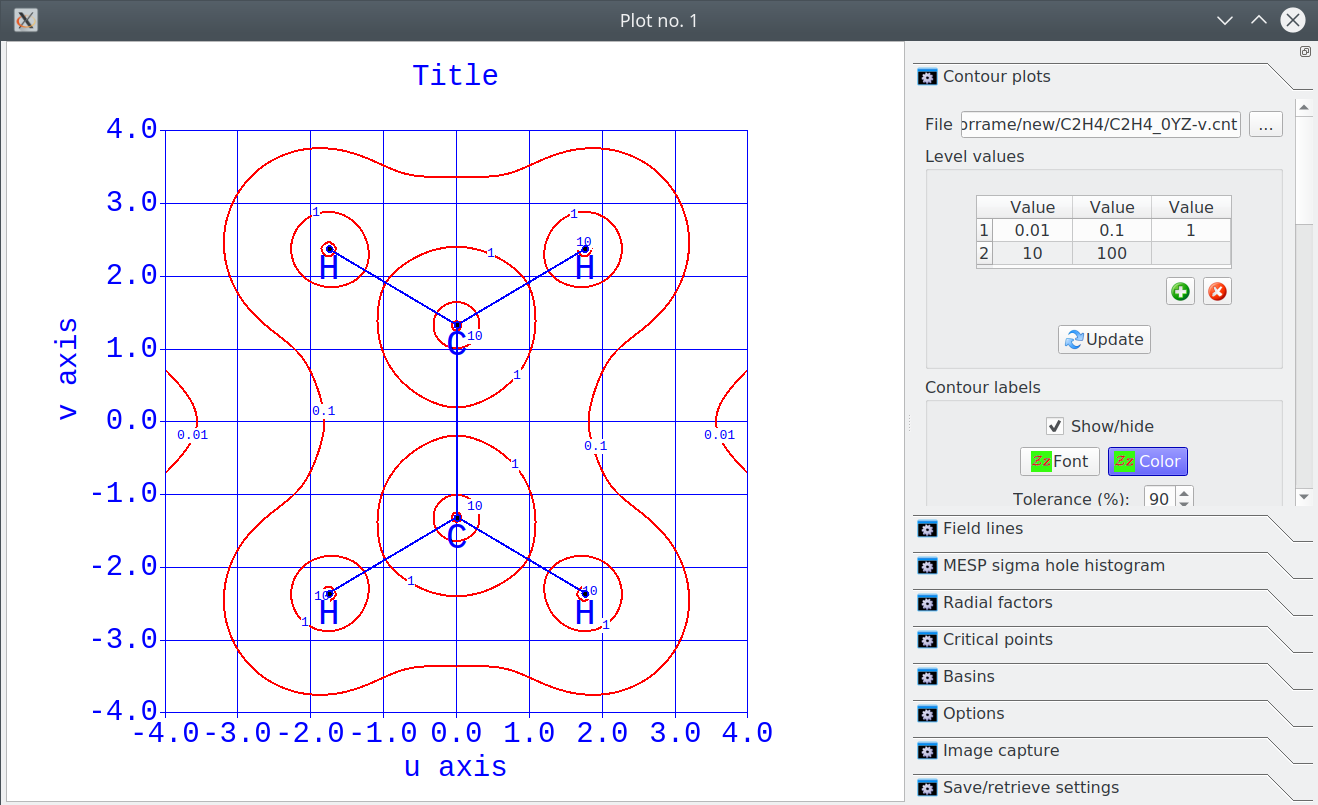
\includegraphics[width=0.95\linewidth]{damqt_QS_fig25.png}
\end{center}
\end{figure} 
\end{minipage}
\begin{minipage}{.5\linewidth}
\begin{figure}[H]
\caption{\label{fig:26}}
\begin{center}
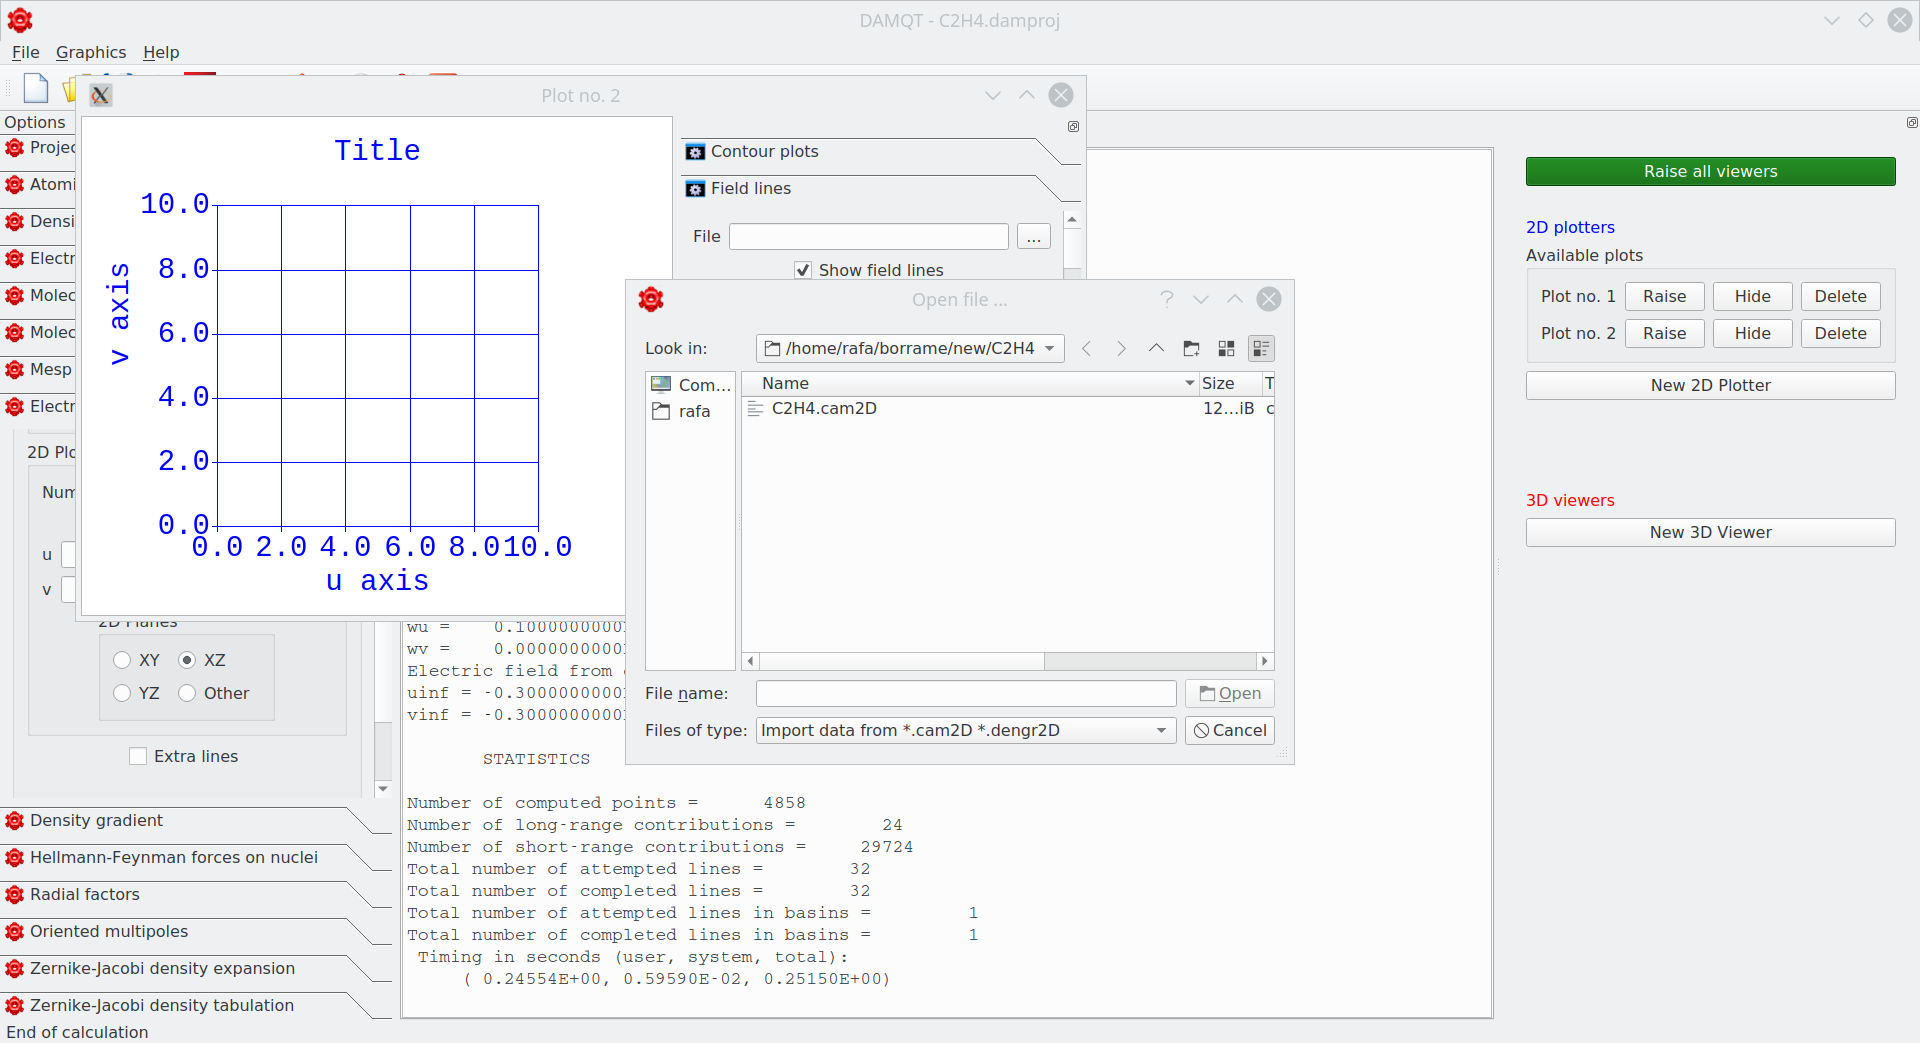
\includegraphics[width=0.95\linewidth]{damqt_QS_fig26.png}
\end{center}
\end{figure} 
\end{minipage}

\begin{minipage}{.5\linewidth}
\begin{figure}[H]
\caption{\label{fig:27}}
\begin{center}
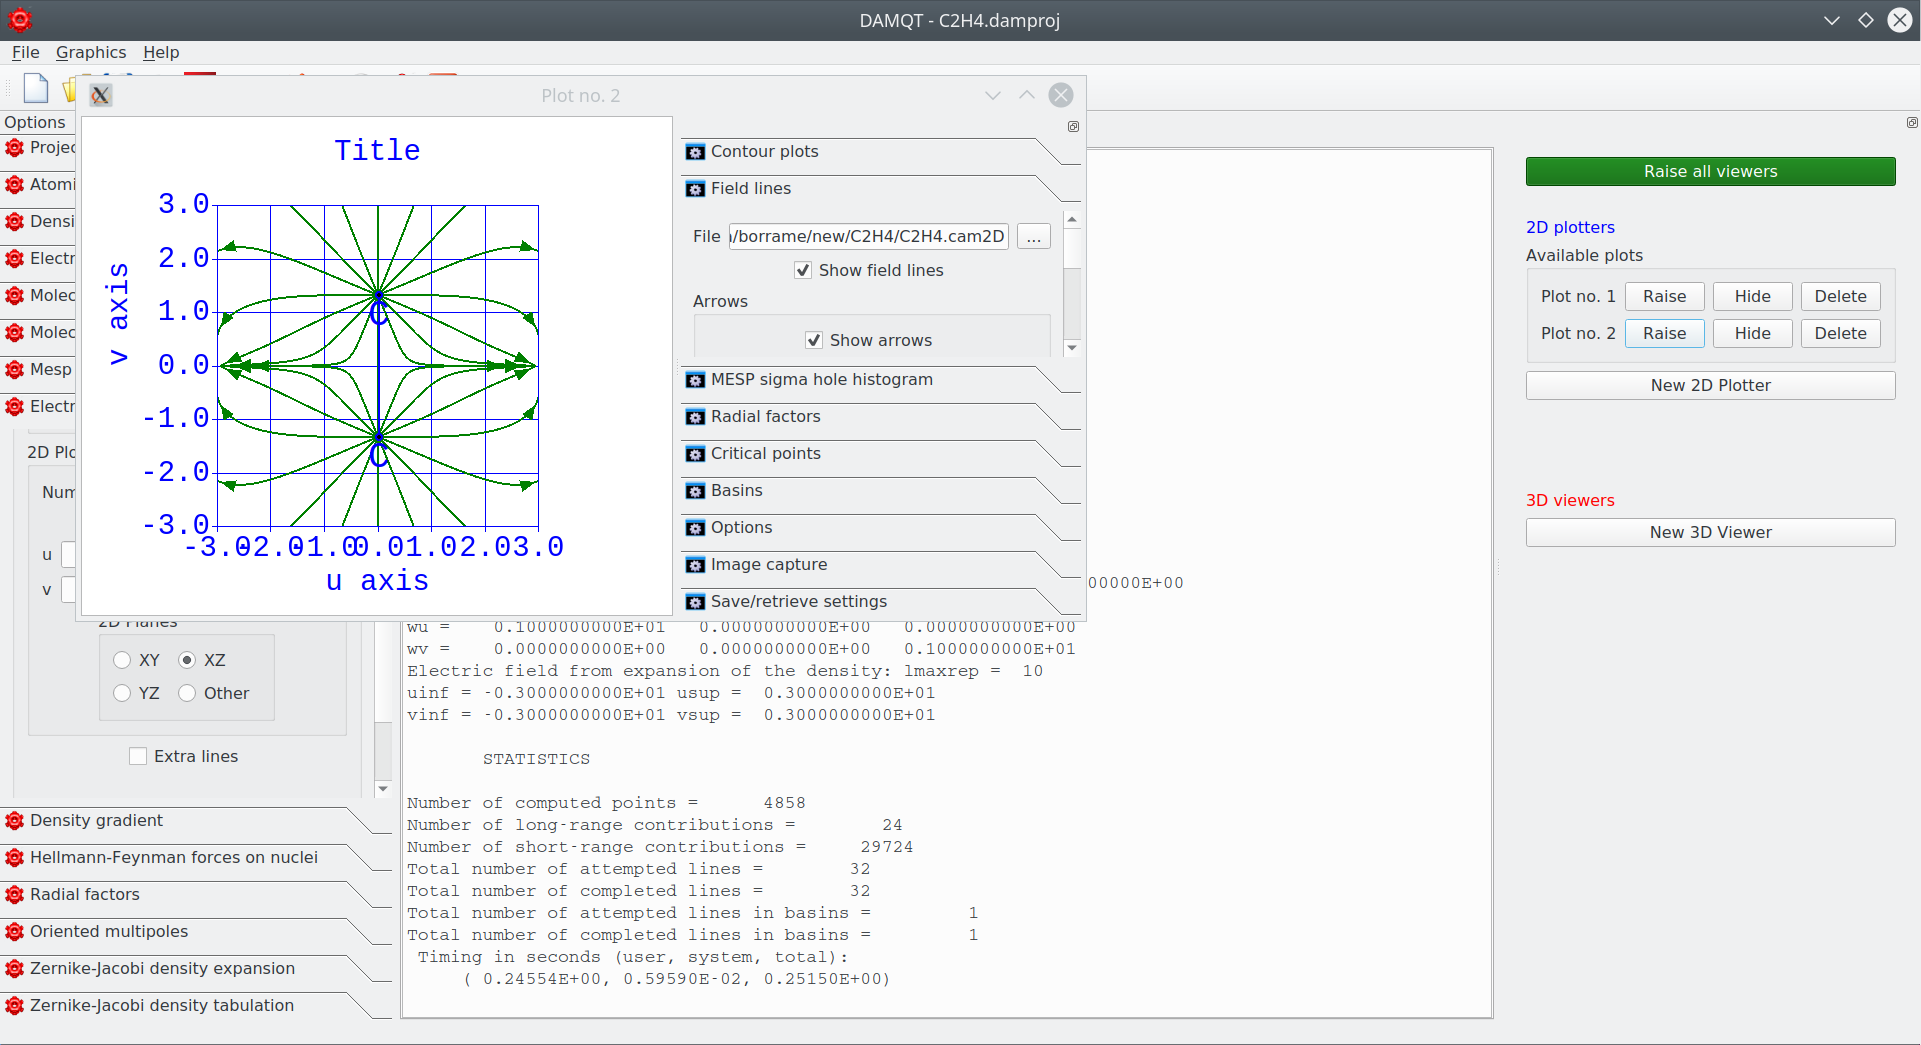
\includegraphics[width=0.95\linewidth]{damqt_QS_fig27.png}
\end{center}
\end{figure} 
\end{minipage}
\begin{minipage}{.5\linewidth}
\begin{figure}[H]
\caption{\label{fig:28}}
\begin{center}
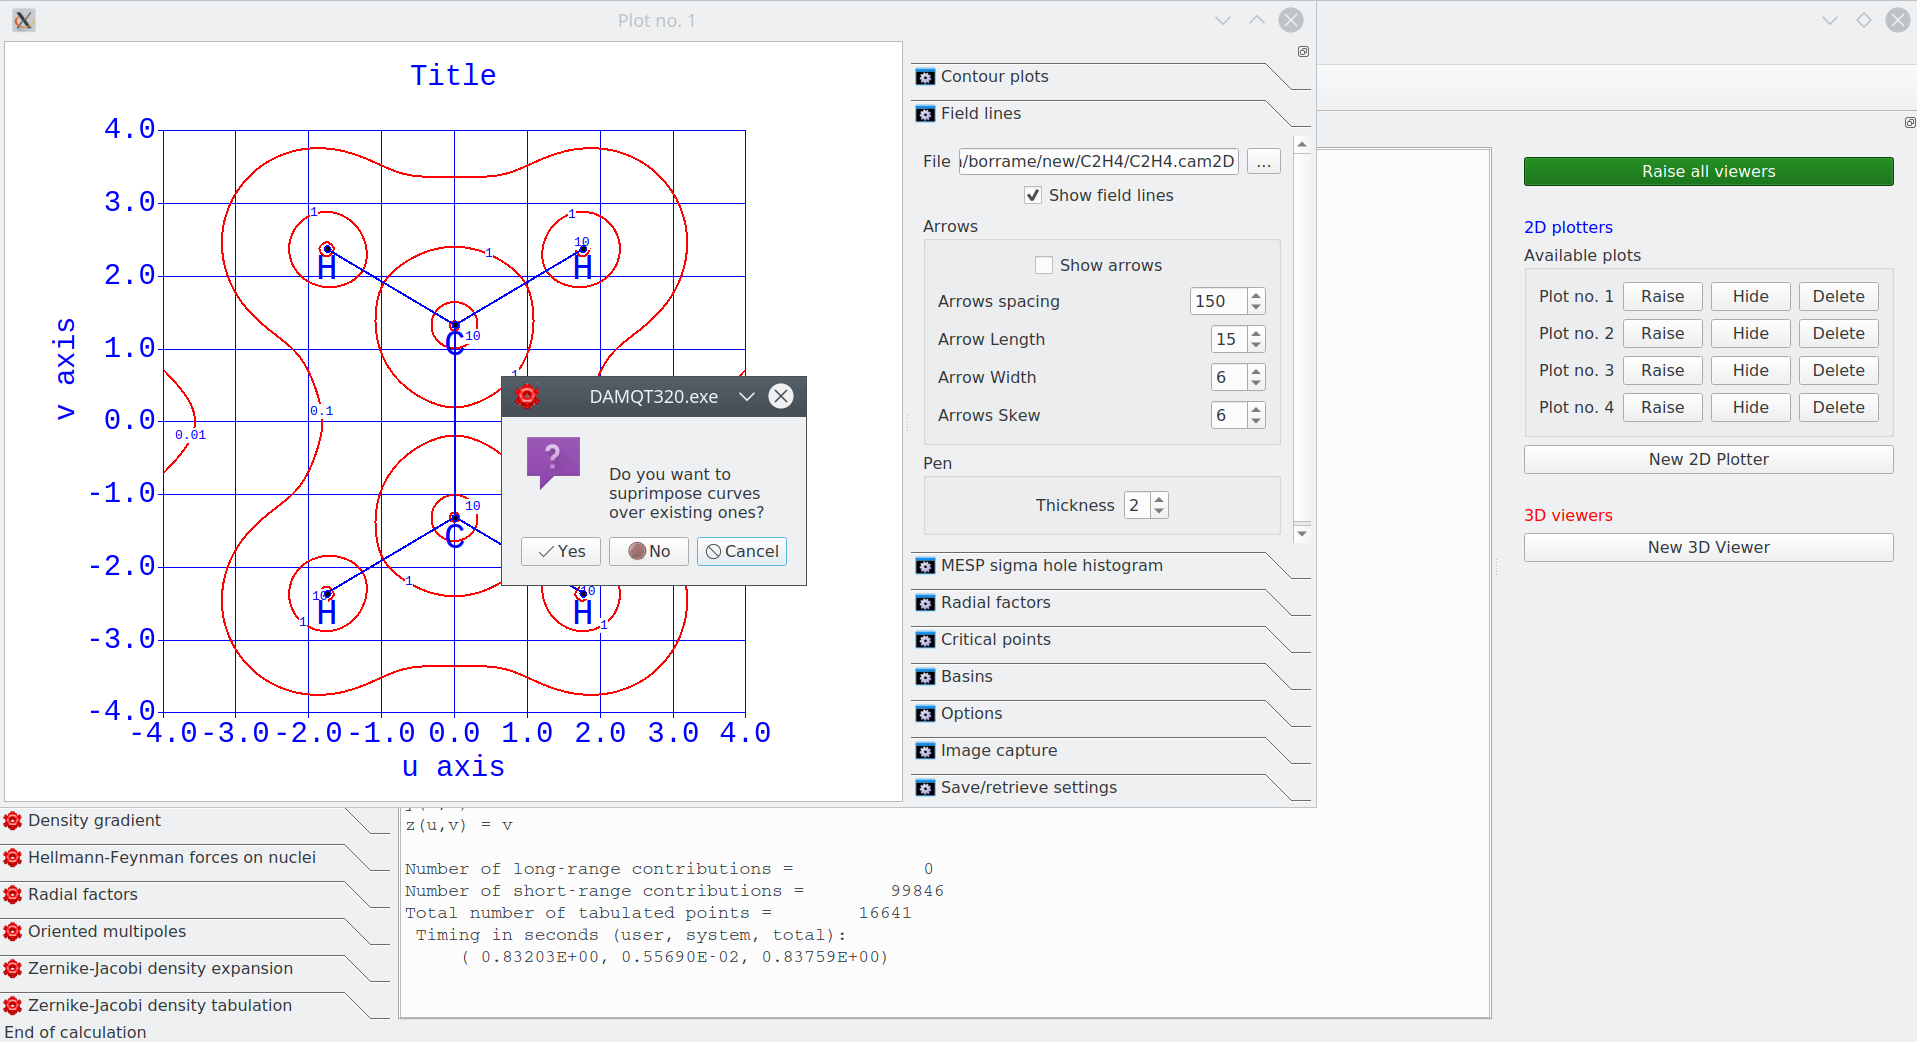
\includegraphics[width=0.95\linewidth]{damqt_QS_fig28.png}
\end{center}
\end{figure} 
\end{minipage}

\begin{minipage}{.5\linewidth}
\begin{figure}[H]
\caption{\label{fig:29}}
\begin{center}
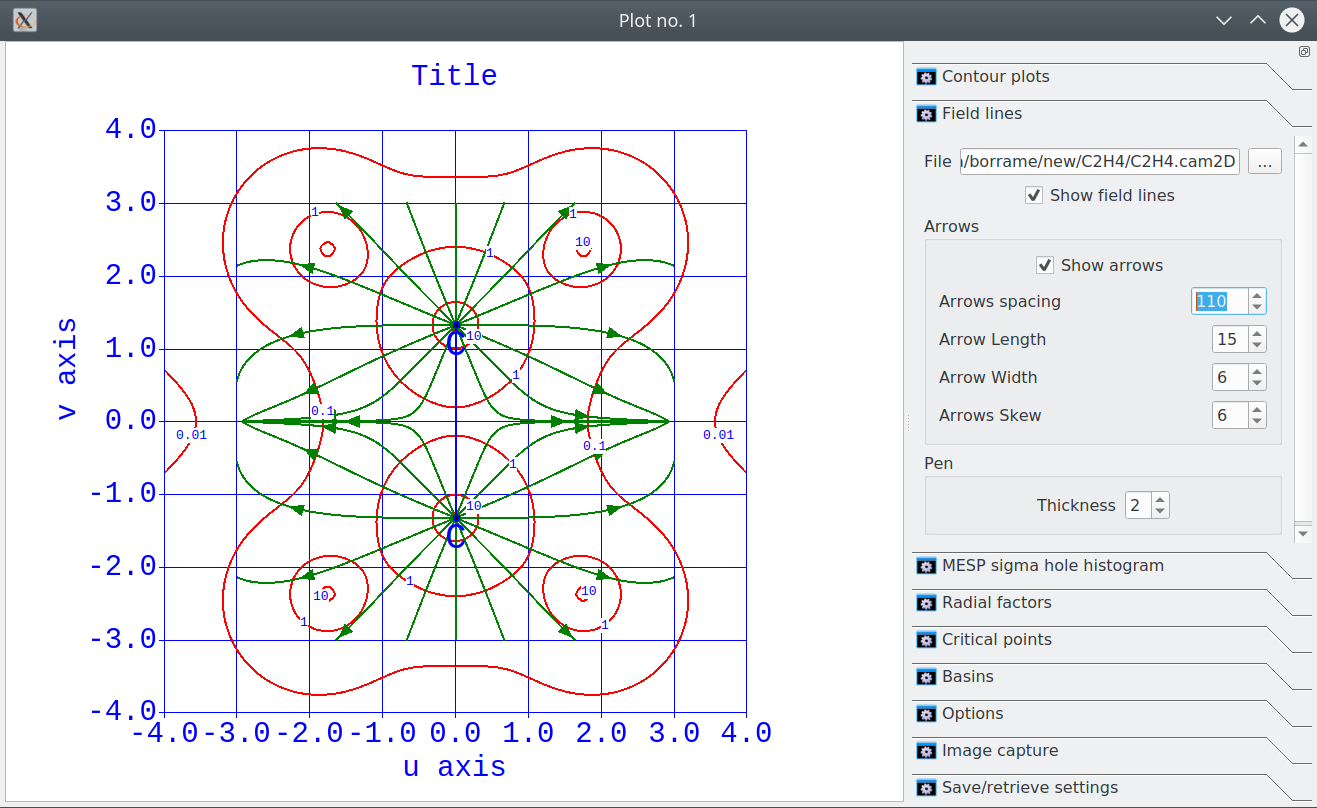
\includegraphics[width=0.89\linewidth]{damqt_QS_fig29.png}
\end{center}
\end{figure} 
\end{minipage}
\begin{minipage}{.5\linewidth}
\begin{figure}[H]
\caption{\label{fig:30}}
\begin{center}
\includegraphics[width=1\linewidth]{damqt_QS_fig30.png}
\end{center}
\end{figure} 
\end{minipage}

\begin{minipage}{.5\linewidth}
\begin{figure}[H]
\caption{\label{fig:31}}
\begin{center}
\includegraphics[width=0.95\linewidth]{damqt_QS_fig31.png}
\end{center}
\end{figure} 
\end{minipage}
\begin{minipage}{.5\linewidth}
\begin{figure}[H]
\caption{\label{fig:32}}
\begin{center}
\includegraphics[width=0.95\linewidth]{damqt_QS_fig32.png}
\end{center}
\end{figure} 
\end{minipage}

\begin{minipage}{.5\linewidth}
\begin{figure}[H]
\caption{\label{fig:33}}
\begin{center}
\includegraphics[width=0.95\linewidth]{damqt_QS_fig33.png}
\end{center}
\end{figure} 
\end{minipage}
\begin{minipage}{.5\linewidth}
\begin{figure}[H]
\caption{\label{fig:34}}
\begin{center}
\includegraphics[width=0.95\linewidth]{damqt_QS_fig34.png}
\end{center}
\end{figure} 
\end{minipage}

\begin{minipage}{.5\linewidth}
\begin{figure}[H]
\caption{\label{fig:35}}
\begin{center}
\includegraphics[width=0.95\linewidth]{damqt_QS_fig35.png}
\end{center}
\end{figure} 
\end{minipage}
\begin{minipage}{.5\linewidth}
\begin{figure}[H]
\caption{\label{fig:36}}
\begin{center}
\includegraphics[width=0.95\linewidth]{damqt_QS_fig36.png}
\end{center}
\end{figure} 
\end{minipage}

\begin{minipage}{.5\linewidth}
\begin{figure}[H]
\caption{\label{fig:37}}
\begin{center}
\includegraphics[width=0.95\linewidth]{damqt_QS_fig37.png}
\end{center}
\end{figure} 
\end{minipage}
\begin{minipage}{.5\linewidth}
\begin{figure}[H]
\caption{\label{fig:38}}
\begin{center}
\includegraphics[width=0.95\linewidth]{damqt_QS_fig38.png}
\end{center}
\end{figure} 
\end{minipage}

\begin{minipage}{.5\linewidth}
\begin{figure}[H]
\caption{\label{fig:39}}
\begin{center}
\includegraphics[width=0.95\linewidth]{damqt_QS_fig39.png}
\end{center}
\end{figure} 
\end{minipage}
\begin{minipage}{.5\linewidth}
\begin{figure}[H]
\caption{\label{fig:40}}
\begin{center}
\includegraphics[width=0.95\linewidth]{damqt_QS_fig40.png}
\end{center}
\end{figure} 
\end{minipage}

\begin{minipage}{.5\linewidth}
\begin{figure}[H]
\caption{\label{fig:41}}
\begin{center}
\includegraphics[width=0.95\linewidth]{damqt_QS_fig41.png}
\end{center}
\end{figure} 
\end{minipage}
\begin{minipage}{.5\linewidth}
\begin{figure}[H]
\caption{\label{fig:42}}
\begin{center}
\includegraphics[width=0.95\linewidth]{damqt_QS_fig42.png}
\end{center}
\end{figure} 
\end{minipage}

\begin{minipage}{.5\linewidth}
\begin{figure}[H]
\caption{\label{fig:43}}
\begin{center}
\includegraphics[width=0.95\linewidth]{damqt_QS_fig43.png}
\end{center}
\end{figure} 
\end{minipage}
\begin{minipage}{.5\linewidth}
\begin{figure}[H]
\caption{\label{fig:44}}
\begin{center}
\includegraphics[width=0.95\linewidth]{damqt_QS_fig44.png}
\end{center}
\end{figure} 
\end{minipage}

\begin{minipage}{.5\linewidth}
\begin{figure}[H]
\caption{\label{fig:45}}
\begin{center}
\includegraphics[width=0.95\linewidth]{damqt_QS_fig45.png}
\end{center}
\end{figure} 
\end{minipage}
\begin{minipage}{.5\linewidth}
\begin{figure}[H]
\caption{\label{fig:46}}
\begin{center}
\includegraphics[width=0.95\linewidth]{damqt_QS_fig46.png}
\end{center}
\end{figure} 
\end{minipage}

\begin{minipage}{.5\linewidth}
\begin{figure}[H]
\caption{\label{fig:47}}
\begin{center}
\includegraphics[width=0.95\linewidth]{damqt_QS_fig47.png}
\end{center}
\end{figure} 
\end{minipage}
\begin{minipage}{.5\linewidth}
\begin{figure}[H]
\caption{\label{fig:48}}
\begin{center}
\includegraphics[width=0.95\linewidth]{damqt_QS_fig48.png}
\end{center}
\end{figure} 
\end{minipage}

\begin{minipage}{.5\linewidth}
\begin{figure}[H]
\caption{\label{fig:49}}
\begin{center}
\includegraphics[width=0.95\linewidth]{damqt_QS_fig49_b.png}
\end{center}
\end{figure} 
\end{minipage}
\begin{minipage}{.5\linewidth}
\begin{figure}[H]
\caption{\label{fig:50}}
\begin{center}
\includegraphics[width=0.95\linewidth]{damqt_QS_fig50_b.png}
\end{center}
\end{figure} 
\end{minipage}

\begin{minipage}{.5\linewidth}
\begin{figure}[H]
\caption{\label{fig:51}}
\begin{center}
\includegraphics[width=0.95\linewidth]{damqt_QS_fig51_b.png}
\end{center}
\end{figure} 
\end{minipage}
\begin{minipage}{.5\linewidth}
\begin{figure}[H]
\caption{\label{fig:52}}
\begin{center}
\includegraphics[width=0.95\linewidth]{damqt_QS_fig52_b.png}
\end{center}
\end{figure} 
\end{minipage}

\begin{minipage}{.5\linewidth}
\begin{figure}[H]
\caption{\label{fig:53}}
\begin{center}
\includegraphics[width=0.95\linewidth]{damqt_QS_fig53_b.png}
\end{center}
\end{figure} 
\end{minipage}
\begin{minipage}{.5\linewidth}
\begin{figure}[H]
\caption{\label{fig:54}}
\begin{center}
\includegraphics[width=0.95\linewidth]{damqt_QS_fig54.png}
\end{center}
\end{figure} 
\end{minipage}

\begin{minipage}{.5\linewidth}
\begin{figure}[H]
\caption{\label{fig:55}}
\begin{center}
\includegraphics[width=0.95\linewidth]{damqt_QS_fig55_b.png}
\end{center}
\end{figure} 
\end{minipage}
\begin{minipage}{.5\linewidth}
\begin{figure}[H]
\caption{\label{fig:56}}
\begin{center}
\includegraphics[width=0.95\linewidth]{damqt_QS_fig56_b.png}
\end{center}
\end{figure} 
\end{minipage}

\begin{minipage}{.5\linewidth}
\begin{figure}[H]
\caption{\label{fig:57}}
\begin{center}
\includegraphics[width=0.95\linewidth]{damqt_QS_fig57_b.png}
\end{center}
\end{figure} 
\end{minipage}
\begin{minipage}{.5\linewidth}
\begin{figure}[H]
\caption{\label{fig:58}}
\begin{center}
\includegraphics[width=0.95\linewidth]{damqt_QS_fig58_b.png}
\end{center}
\end{figure} 
\end{minipage}

\begin{minipage}{.5\linewidth}
\begin{figure}[H]
\caption{\label{fig:59}}
\begin{center}
\includegraphics[width=0.95\linewidth]{damqt_QS_fig59_b.png}
\end{center}
\end{figure} 
\end{minipage}
\begin{minipage}{.5\linewidth}
\begin{figure}[H]
\caption{\label{fig:60}}
\begin{center}
\includegraphics[width=0.95\linewidth]{damqt_QS_fig60_b.png}
\end{center}
\end{figure} 
\end{minipage}

\begin{minipage}{.5\linewidth}
\begin{figure}[H]
\caption{\label{fig:61}}
\begin{center}
\includegraphics[width=0.95\linewidth]{damqt_QS_fig61_b.png}
\end{center}
\end{figure} 
\end{minipage}
\begin{minipage}{.5\linewidth}
\begin{figure}[H]
\caption{\label{fig:62}}
\begin{center}
\includegraphics[width=0.95\linewidth]{damqt_QS_fig62_b.png}
\end{center}
\end{figure} 
\end{minipage}

% \begin{minipage}{.5\linewidth}
% \begin{figure}[H]
% \caption{\label{fig:28}}
% \begin{center}
% \includegraphics[width=0.95\linewidth]{damqt_QS_fig36.png}
% \end{center}
% \end{figure} 
% \end{minipage}

\end{document}
